%%% PREAMBLE
\documentclass[11pt,titlepage,oneside]{book}
\usepackage{tablefootnote}
\usepackage{float}
\usepackage[lmargin=1in,rmargin=1in,tmargin=1in,bmargin=1in]{geometry} % see geometry.pdf on how to lay out the page. There's lots.
\geometry{a4paper}

%%%%%% FOR TESTING ONLY %%%%%%%%%%%%%
\usepackage[english]{babel}
%%%%%%%%%%%%%%%%%%%%%%%%%%%%%%

%%%%%%%%%%%%%%%%% PACKAGES %%%%%%%%%%%%%%%%%

\usepackage{graphicx} % enhanced grpahics support
\renewcommand{\sfdefault}{cmbr} % slightly nicer than the standard sans serif font
\usepackage[onehalfspacing]{setspace} % line spacing
\usepackage[T1]{fontenc} % font encoding (fixes some font-related errors)
\usepackage{textcomp} % more font encoding
\usepackage[printonlyused]{acronym} % To handle acronyms
\usepackage{appendix} % For managing appendices (makes ToC neater)
\usepackage{fancyref}

%%%%%%%%%%%%%%%%% DOCUMENT PROPERTIES %%%%%%%%%%%%%%%%%

% Thesis details
\newcommand{\LongTitle}{Collaborative-Based Filtering Music Reccomendation System for DJ Sets}
\newcommand{\Me}{Harvey James Prewer}

% Number of document levels
\setcounter{secnumdepth}{4}

% Prevent hyphenation
\hyphenpenalty=5000
\tolerance=1000

%%%%%%%%%%%%%%%%% ACRONYMS AND SYMBOLS %%%%%%%%%%%%%%%%%

\newcommand{\RT}{RT\ensuremath{_{\text{60}}}}
\newcommand{\DEG}{\ensuremath{^\circ}}

%%%%%%%%%%%%%%%%% DATE %%%%%%%%%%%%%%%%%

% For placing on title page
\usepackage{datetime}
\newdateformat{MyMonth}{\monthname[\THEMONTH]}
\newdateformat{MyYear}{\THEYEAR}
\newdateformat{MyDate}{\THEYEAR}

%%%%%%%%%%%%%%%%% CAPTIONS %%%%%%%%%%%%%%%%%

\usepackage[margin=2em,singlelinecheck=on,font=sf,labelfont+=bf,labelformat=simple,labelsep=colon]{caption}

\newcommand{\captionfontsize}{\fontsize{9}{11}\selectfont}
\renewcommand\captionfont{\captionfontsize\sffamily}

%%%%%%%%%%%%%%%%% TITLES %%%%%%%%%%%%%%%%%

\usepackage[sf,raggedright,toctitles]{titlesec}

% Chapter heading properties
\titlespacing{name=\chapter}{0ex}{0ex}{.5in}[0ex]
\titlespacing{name=\chapter,numberless}{0ex}{0ex}{.5in}[0ex]

% Subsubsection heading properties
\titleformat{name=\subsubsection,numberless}[hang]{\sf}{}{0pt}{\bfseries}
\titlespacing{name=\subsubsection,numberless}{0em}{2ex}{0ex}

%%%%%%%%%%%%%%%%% TOC / LOF / LOT / LOE %%%%%%%%%%%%%%%%%

\usepackage[titles]{tocloft}

\setcounter{lofdepth}{1}

% put "Chapter #: " in ToC
\renewcommand{\cftchappresnum}{\chaptername~}
\renewcommand{\cftchapaftersnum}{:}
\newlength{\mylen} % a "scratch" length
\settowidth{\mylen}{\bfseries\chaptername\cftchapaftersnum} % extra space
\addtolength{\cftchapnumwidth}{\mylen} % add the extra space

% control indention
\setlength{\cftchapindent}{0em}
\setlength{\cftfigindent}{0em}
\setlength{\cfttabindent}{0em}

\newlength{\tocloftindent}
\setlength{\tocloftindent}{2.3em}

\setlength{\cftsecindent}{1.5em}

%\renewcommand{\@pnumwidth}{1.9em} % was 1.55em
%\renewcommand{\@tocrmarg}{2.9em plus1fil} % raggedright toc entries (no hyphenation)

\setlength{\cftsubsecindent}{3.8em}

%%%%%%%%%%%%%%%%% TABLES %%%%%%%%%%%%%%%%%

\usepackage{array,color,colortbl,multirow,longtable}

\newcommand{\colheading}[1]{\multirow{2}{*}{\textbf{#1}}} % custom column heading command
\newcommand{\tablesubtitle}[2]{\multicolumn{#1}{l}{\emph{#2}}} % custom table sub heading to span the specified number of columns
\renewcommand\arraystretch{1.2} % row height

%%%%%%%%%%%%%%%%% MATHS %%%%%%%%%%%%%%%%%

\usepackage{amsmath,amsbsy,amssymb}

\allowdisplaybreaks

% define new symbols and operators
\newcommand{\R}{\mathfrak{R}} % Real operator
\newcommand{\Z}{\mathbb{Z}} % set of integers
\newcommand{\N}{\mathbb{N}} % set of natural numbers
\newcommand{\F}{\mathcal{F}} % Fourier operator
\newcommand{\ud}{\,\text{d}} % d in differential
\newcommand{\fs}{f\negthinspace{}s} % sampling frequency
\DeclareMathOperator*{\argmax}{arg\,max} % arg min
\DeclareMathOperator*{\argmin}{arg\,min} % arg max
\providecommand{\abs}[1]{\lvert#1\rvert} % abs brackets

%%%%%%%%%%%%%%%%% CITATIONS %%%%%%%%%%%%%%%%%

\usepackage[round]{natbib}

\setcitestyle{aysep={,},notesep={: },citesep={;},yysep={,}}
%\setcitestyle{authoryear,open={(},close={)}}

\setlength{\bibhang}{0pt}

\newcommand{\citepos}[1]{\citeauthor{#1}'s \citeyearpar{#1}}
\newcommand{\citequote}[1]{\newline \strut\hfill \citep{#1}}
\newcommand{\cpage}[1]{p.~#1}
\newcommand{\cpages}[2]{pp.~#1--#2}
\renewcommand\bibname{References}

%%%%%%%%%%%%%%%%% HEADER/FOOTER %%%%%%%%%%%%%%%%%

\usepackage{fancyhdr}
\setlength{\headheight}{15pt}

\newcommand{\myfooter}{\textsf{\thepage}}

\fancypagestyle{plain}{%
	\fancyhf{}%
	\fancyfoot[R]{\myfooter}%
	\renewcommand{\headrulewidth}{0pt}%
	\renewcommand{\footrulewidth}{1pt}%
}

\pagestyle{fancy}
\fancyhf{}%
\renewcommand{\headrulewidth}{1pt} %header line width
\renewcommand{\footrulewidth}{1pt} % footer rule width
\fancyhead[R]{\textsf{\nouppercase{\leftmark}}} % header right - chapter title
\fancyfoot[R]{\myfooter} % footer right - page number

%%%%%%%%%%%%%%%%% HYPERREF %%%%%%%%%%%%%%%%%

% this should hopefully be the last entry in the preamble - defines properties of the typeset pdf file
% this package makes clickable links in the pdf
\usepackage[colorlinks,breaklinks,pdfdisplaydoctitle,plainpages=false]{hyperref} 
\hypersetup{pdftitle={\LongTitle},pdfauthor={\Me},
	citecolor=black,%
	filecolor=black,%
	linkcolor=black,%
	urlcolor=black
}

\renewcommand{\equationautorefname}{Equation}
\renewcommand{\figureautorefname}{Figure}
\renewcommand{\Itemautorefname}{Item}
\renewcommand{\tableautorefname}{Table}
\renewcommand{\sectionautorefname}{Section}
\renewcommand{\subsectionautorefname}{Section}
\renewcommand{\subsubsectionautorefname}{Section}
\renewcommand{\chapterautorefname}{Chapter}
\renewcommand{\partautorefname}{Part}

%%%%%%%%%%%%%%%%%%%%%%%%%%%%%%%%%%%%%%%%%%%%
%%%%%%%%%%%%%%%%% DOCUMENT %%%%%%%%%%%%%%%%%
%%%%%%%%%%%%%%%%%%%%%%%%%%%%%%%%%%%%%%%%%%%%

\begin{document}
	
	\pdfbookmark[0]{Title page}{title} % Sets a PDF bookmark for the title page
	\setlength{\parindent}{0pt} % set paragraph indent
	\setlength{\parskip}{0ex} % set paragraph spacing
	\pagenumbering{alph} % prevents warnings about duplicated page numbering
	
	% !TEX root = ../TechProject.tex

\graphicspath{{FrontMatter/}}

%%%%%%%%%%%%%%%%% TITLE PAGE %%%%%%%%%%%%%%%%%
\begin{titlepage}
\thispagestyle{empty}
\hfill\includegraphics[width=50mm]{images/UniS_Logo.pdf}
{\sf
\centering
\null\vfil\vfil
	{
		\huge\LongTitle\\
	}
\vfil\vfil\vfil
	{
		\Large\Me\\
	}
\vfil\vfil\vfil
	{
		\Large{}BMus/BSc Music \& Sound Recording (Tonmeister)\\
		Technical Project\\
	}
\vfil\vfil
	{
		\Large{}Institute of Sound Recording\\
		University of Surrey\\
	}
\vfil
	{
		\Large\MyMonth\today~\MyYear\today\\}
	}

	{
		\includegraphics[width=40mm]{images/University_of_Surrey_coat_of_arms.pdf}
		\vspace{-.4in}
	}
\end{titlepage}

\setlength{\parskip}{1ex plus 0.2ex minus 0.2ex} % set paragraph spacing
\onehalfspacing

%%%%%%%%%%%%%%%%% ABSTRACT %%%%%%%%%%%%%%%%%

\pdfbookmark[0]{Abstract}{abstract}

\chapter*{Abstract}
\thispagestyle{empty}
\setcounter{page}{2}

Music recommendation systems are used to filter down the vast amount of commercially available music to a digestible and personable amount. Recommendation systems have seen significant improvement recently due to advances in deep learning. However, listeners with diverse musical taste still do not use recommendation systems. This is evident with the continued popularity of internet radio and the desire for "curation" found in streaming services. DJs are in this diverse category, and considering the amount of investigation needed to prepare a DJ set, an algorithmic way of preparing a DJ set is desirable. With the vast amount of DJ sets available online, training a recommendation system on DJ sets could resolve this issue and other DJ-related tasks.

In this project, a novel DJ-set recommendation model is proposed. The model is trained on DJ sets, available on MixesDB, an online database for DJ sets. It makes use of the matrix factorisation algorithm, alternating least squares. The audio features used for this model were obtained from Spotify API and then leveraged to improve suggestions further.

An experiment was also conducted that tests the R-Precision of the application, an evaluation metric used for the million playlist Spotify challenge. An evaluation set was made, and the parameters for obtaining the highest average R-precision were investigated. The proposed model operated successfully; however, compared to the top-performing models, the model underperformed significantly. It's thought that the sparsity of the dataset is the main contributor to its results.

%%%%%%%%%%%%%%%%% ACTUAL FRONT MATTER %%%%%%%%%%%%%%%%%
\frontmatter

\singlespacing

\setlength{\parskip}{0ex} % set paragraph spacing

\clearpage
\pdfbookmark[0]{Contents}{Contents}
\phantomsection
\tableofcontents
\clearpage
\phantomsection
\addcontentsline{toc}{chapter}{List of Figures}
\listoffigures
\clearpage
\phantomsection
\addcontentsline{toc}{chapter}{List of Tables}


\setlength{\parskip}{1ex plus 0.2ex minus 0.2ex} % set paragraph spacing

\onehalfspacing

\chapter{Acknowledgements}

Thanks to Christos for the encouragement and advice whilst doing this. Thank you to my parents and my friends for always being loving and compassionate. Thank you to Malibu for sound-tracking a huge majority of the put into this.
	
	%%%%%%%%%%%%%%%%% MAIN %%%%%%%%%%%%%%%%%
	\mainmatter
	
	% change header
	\renewcommand{\chaptermark}[1]{\markboth{\chaptertitlename\ \thechapter: #1}{}}
	
	\pagenumbering{arabic}
	\setlength\abovedisplayshortskip{0.5\baselineskip}
	\setlength\belowdisplayshortskip{0.5\baselineskip}
	\setlength\abovedisplayskip{0.5\baselineskip}
	\setlength\belowdisplayskip{0.5\baselineskip}
	
	%%%%%%%%%%%%%%%%%%%%%
	%%%%%%%%%%%%%%%%%%%%%
	% For example
	
	%\include{Introduction}
	
	% The argument for \include is a filename of a LaTeX file contained within the same folder at this file. It could also be placed in a subfolder; the argument can then be specified as {subfolder_name/filename}.
	
	% The \include'd file contains LaTeX commands that will, more or less, be read as if the code was contained in this file at the point the \include was called.
	
	% There is an equivalent command, \includeonly, which you should place at the top of your document. Use this command to choose the files to include (rather than commenting lines). In this way, the document will be typeset as if the files were present (so links and cross-references won't be broken), but any output associated with the files will be excluded.
	
	% Another tip: If using TeXShop, which uses synctex, you can command click on the preview to find the corresponding commands in your source. The reverse operation is also permitted. To do this from \include'd files, you need to tell TeXShop what the root file is. This is done by placing this line AT THE TOP of each \include'd file (you must include the "%"):
	% ! TEX root = root_filename.tex
	% Doing this has other advantages, like being able to typeset from an included file, rather than having to typeset from the root file.

% Chapter 1
% !TEX root = ../TechProject.tex

\graphicspath{{Chapter1/}}

% for example

\chapter{Introduction}
With the rise of streaming services found for multiple formats, recommendation systems are applications one interacts with daily. Within the context of music, its a ideal way of filtering the sheer quantity of commercially available music down to a sizeable amount that aligns well with your taste. With the prevalence of machine learning and deep learning, this technology is made advantage of in the current modern day systems provided by services like Spotify. For the majority of listeners automating the discovery process has been well received however a subset of listeners still find these systems inadequate.

Recent studys highlight people with objectively "diverse" music tastes usually rely on non algoritmic ways of finding music. This is apparrent with the withstanding popularity of internet radio and formats like Band-Camp. 

Compared to a standard user, most DJs would fall in the catagory of having a diverse taste and finding songs through these platforms is usually the go-to for preparing a DJ set.

However, with sheer quantity of DJ sets archived, one would suspect that training recommendation system on this data would provide an affectively algorithmic way to suggest music to cater to this specific audience. This paper presents a recommendation system trained on DJ sets, and see if training on a specific dataset could compete with top performing models.

In order to discuss this throrughly, this paper tackles the follwing:

\begin{enumerate}
	\item \textit{What are effective methods for the automated recommendation of songs suitable
		for adding to a given DJ set}
	\item \textit{Is the proposed method a suitable solution to the above question?}
	\item \textit{Can this application be further developed to solve other DJ tasks?}
\end{enumerate}

Chapter 2 and 3 covers a literature review. Chapter 4 will present the gaps in current study's and present a hypothesis. Chapter 5 gives an overview of the application and run through a few example recommendations. Chapter 6 runs through how the application got tested in a methodical way. Chapter 7 goes through the results found and compares it to industry standard models. Chapter 8 concludes the study and discusses further work 
 

% Chapter 2
% !TEX root = ../TechProject.tex

\graphicspath{{Chapter2/}}

\chapter{Machine Learning used in Music Recommendation Systems}

This chapter will answer the following research question:

\textit{What are effective methods for the automated recommendation of songs suitable for adding to a given DJ set?} 

\section{The need for music recommendation systems}
Spotify, SoundCloud, Apple Music and other streaming services give one access to a library of tens of millions songs. Music Recommendation systems are excellent at fitting a user's preference whilst incorporating some level of filtering of an overwhelming amount of songs \citep{bollen_understanding_2010}. 

Music recommendation systems study the habits and tastes of users, and with that information give out suitable recommendations. This aids the listener to discover new songs or artists they otherwise would not have found.

With this potential, a well made recommendation system could be a make or break for choosing one streaming service from another. For this reason a lot of research gets put into recommendation systems as an attempt to retain engagement. 

 With recommending music, a lot of sub conscious factors come into play on what a user wants to listen to at a given time. This can range from characteristics and mood of the listener, to what they get up to in day-to-day life \citep{ferwerda_personality_2015, rentfrow_re_2003, gillhofer_iron_2015, wang_context-aware_2012}.  The users environment can have an affect as well \citep{kaminskas_location-aware_2013}. Observing a user made playlists also can reveal a lot on what groups of songs work for particular situations \citep{zheleva_statistical_2010, mcfee_hypergraph_2012}.
 
 A necessity for making a recommendation system suited for a type of product is taking into consideration the common place attributes of the product. Music lends itself to having a specific method due to short duration and high emotional connection. A recommendation system that uses these attributes to its advantage will be more successful than ones that don't.

\section{Collaborative filtering}

Collaborative filtering guesses a user's taste by looking at similar user-item connections. Using an explicit example, if a user rates something highly, it can provide similar suggestions from looking at the ratings of other users\citep{celma_recommendation_2010}.

\begin{figure}[H]
	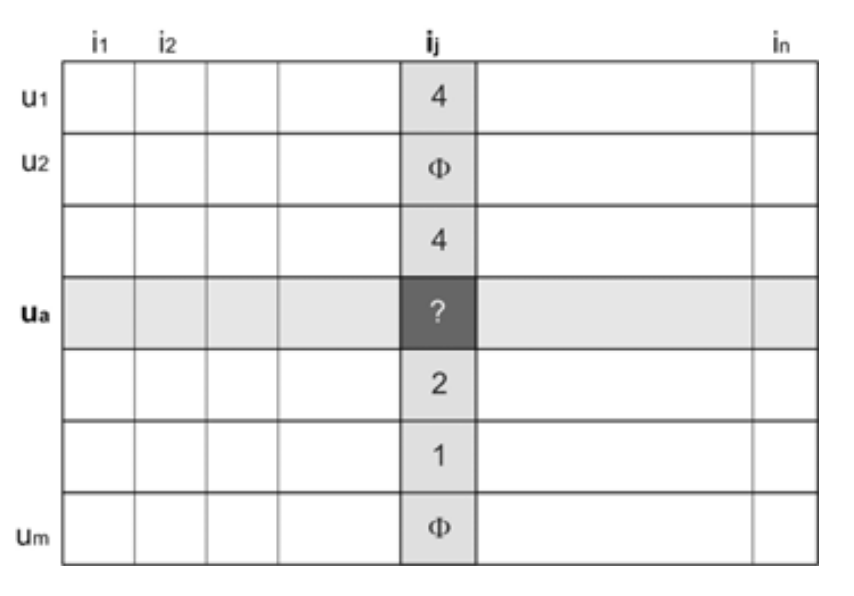
\includegraphics[scale=0.65]{images/collaborative_filtering}
	\centering
	\caption{User-item matrix used for collaborative filtering \citep{celma_recommendation_2010}} 
	\label{fig:figure}
\end{figure}

Collaborative filtering works by taking a matrix of users and items where some form of interaction is measured. Examples of interaction's could be plays of a song, rating of a movie/product or screen time on an app. In figure 2.1, i represents items, and u is users.

The first known use of collaborative filtering is with Goldberg's "Tapestry" system, a mailing list filter where users collectively decide which type of emails get the most importance \citep{goldberg_using_1992}. The first instance of collaborative filtering being used for music recommendations was in a system called Ringo where users would rate music (album, songs, artists, etc.) and get recommendations pulled from similar users \citep{shardanand_social_1995}. 

Despite the prevalence of deep learning and neural networks, collaborative filtering is still used in today's state of the art recommendation systems. The winner of the 2018  RecSys Playlist Continuer Challenge used a combination of collaborative filtering and deep learning in their model \citep{volkovs_two-stage_2018}.

Collaborative filtering can be divided into the following types:

\begin{enumerate}
	\item Explicit Feedback
	\item Implicit Feedback
	\item Item Based
	\item User Based
\end{enumerate}




\subsection{Explicit Feedback}

 Explicit feedback is when a user is asked for some form of measurement about the likeability of a product \citep{celma_recommendation_2010}. The RACOFI (Rule-Applying Collaborative Filtering) system uses explicit feedback. Collaborative filtering with ratings finds initial recommendations. Then the system applies logic rules to decipher further the most suitable recommendations \citep{anderson_racofi_2003}.  Its added logic rules implicitly change the user’s previous ratings. Other recommendation systems started having similar rules, including Indiscover and Slope One \citep{celma_music_2010, lemire_slope_2007}. Ringo and many of the first music recommendation systems that use collaborative filtering use explicit feedback for their data. 

\subsection{Implicit Feedback}

Recommendation systems that take only implicit feedback will focus on what the listener interacts with, rather than asking them for their opinion of the content. The main reason implicit feedback is frowned upon is that using this method doesn't give a scale of enjoyability of the content, in the context of music, just whether the user listened to said song or artist how many times \citep{celma_recommendation_2010}. Spotify is an example of this, if another person uses their account or if they left a device on autoplay as well on mute. However, collecting implicit data is a lot easier because it just requires engagement with the said application to get valuable information. 

There is also a lot to be found with implicit data. In 2018, a music recommendation system produced an effective recommendations derived from the time of day in which users listened to music \citep{sanchez-moreno_incorporating_2018}. Takama et al took this a step further by using time of day as well as, nationality and content features found through Spotify \citep{takama_context-aware_2021} 

\subsection{Item-Based Neighbourhood }

Item-based neighbourhood is when similarities for a given item are found based on the user's previous item ratings. First one calculates the similarity among the item's ratings and then the prediction of a given items rating is calculated. Figure 2.2 shows a matrix with ratings from  $u_{2}, u_{i}$ and $u_{m-1}$. For finding similarities between $i_{i}$ and $i_{k}$, we only take $u_{2}$ and  $u_{i}$ into consideration when using item based neighbourhood because they have rated both item $i_{i}$ and $i_{k}$.  

\begin{figure}[H]
	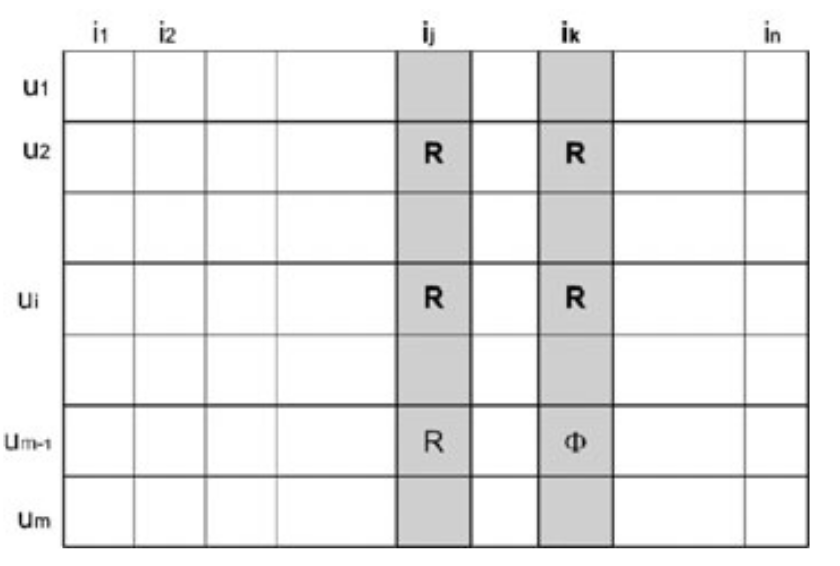
\includegraphics[scale=0.65]{images/neigbourhood_based}
	\centering
	\caption{Matrix showing given ratings. \citep{celma_recommendation_2010}} 
\end{figure}

There are many ways to calculate how similar two items, examples being cosine similarity, Pearson correlation or adjusted cosine similarity. Equation 2.1 shows cosine similarity, the inner product space is taken into account by calculating its similarity.

\begin{equation}
		sim(i , j) = cos( \textbf{i}, \textbf{j} ) = \frac{ \textbf{ i }, \textbf{ j }}{ || i || * || j || } = \frac{ \sum_{ u \in U } r_{ u, i }, r_{ u, j }} { \sqrt{ \sum _{  u \in U } r^{2}_{ u , i}} \sqrt{ \sum _{  u \in U } r^{2}_{ u , j}}}
\end{equation}

Cosine similarity is not advised for comparing how similar recommendations are because users often have their own personal ranges when it comes to rating. Adjusted cosine similarity is good because it subtracts the users average from each co-rated pair, this handles users personal ranges appropriately \citep{sarwar_item-based_2001}. Equation 2.2 for adjusted cosine similarity is shown.

\begin{equation}
	sim(i , j) = \frac{ \sum_{ u \in U } ( r _{ u, i } - \bar{r} _{u} ) ( r _{ u, j} - \bar{r} _{u} ) } { \sqrt{\sum_{ u \in U } ( r _{ u, i } - \bar{r} _{u} )^2} \sqrt{\sum_{ u \in U } ( r _{ u, j } - \bar{r} _{u} )^2}}
\end{equation}

Once similarities of the users previous ratings are calculated, the next step is to predict how the user would rate the item in question. A way of doing this is to calculate a weighted sum of the user's previous item ratings. Calculating the weighted sum predicts how the user would rate the given item based on the ratings of similar items. Weighted sum is scaled to ensure the predicted rating is in an appropriate range\citep{sarwar_item-based_2001}. Allowing $ S^{k}(i;u)$ to equal the list of items i user u has rated, equation 2.3 shows how the predicted value is found.

\begin{equation}
	\hat{r} _{u,i} = \frac{ \sum _{ j \in S^{k}(i;u)} sim(i , j) r _{u, j}}{\sum _{j \in S^{k}(i;u)} sim(i , j)}
\end{equation}
\\
\\
\\
Another way of predicting a rating is using Regression. Predictions are made with the same equation as weighted sums, but approximate values based on a linear regression model are used instead of "raw" rating values. Allowing target items be \textit{i} and similar item N by $R_{i}$ and $R_{N}$, 2.4 shows the linear regression model \citep{sarwar_item-based_2001}.

\begin{equation}
	\bar{R'} _{N} = \alpha \bar{R}_{i} + \beta + \varepsilon
\end{equation}

Parameters of the regression model ($\alpha , \beta$) are found by going through the rating vector pairs, and $\varepsilon$ is the error of the model \citep{sarwar_item-based_2001}.

\subsection{User Based}

User-based neighbourhood is when you look for users who rate similarly to see whether item i is similar to user u. This differs from Item Based because user based skips calculating similarity of co-rated items \citep{pinela_recommender_2017}. Equation 2.5 shown is similar to 2.3 but instead it sums a list of similar users.

\begin{equation}
	\hat{r} _{u,i} = \bar{r}_{u} + \frac{ \sum _{v \in S(u)^{k}} sim(u ,v) ( r_{v, i} - \bar{r}_{v})}{\sum _{v \in S(u)^{k}} sim(u , v)}
\end{equation}

As mentioned previously, pearson correlation, cosine similarity can be used to calculate similarity ($sim(u ,v)$). Another way of calculating similarity is matrix factorisation

\subsection{Matrix Factorisation}

\begin{figure}[H]
	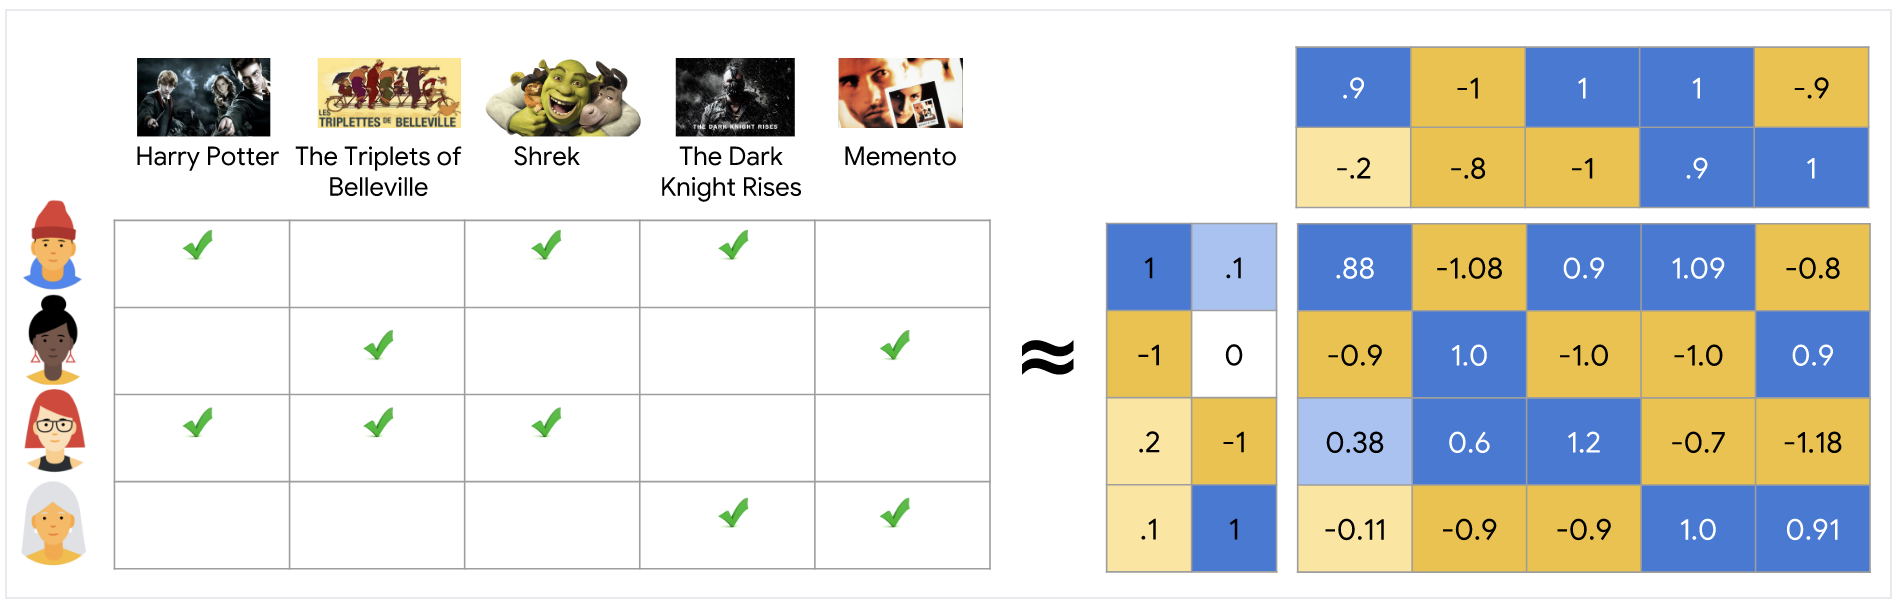
\includegraphics[scale=0.45]{images/matrix_factorisation_example}
	\centering
	\caption{A Movie Rating example of matrix factorisation  \citep{httpsdevelopersgooglecom_matrix_2023}} 
	\label{fig:figure}
\end{figure}

When one has a matrix of plays for each user and song, matrix factorisation can be used to find recommended songs. Matrix factorisation processes the matrix into 2 vectors. These vectors are from factors of the user item rating patterns \citep{koren_matrix_2009}. Figure 2.3 and 2.4 illustrates how, where latent factors (products used to factorise matrix) are used to approximate and predict users ratings of movies. 

\begin{figure}[H]
	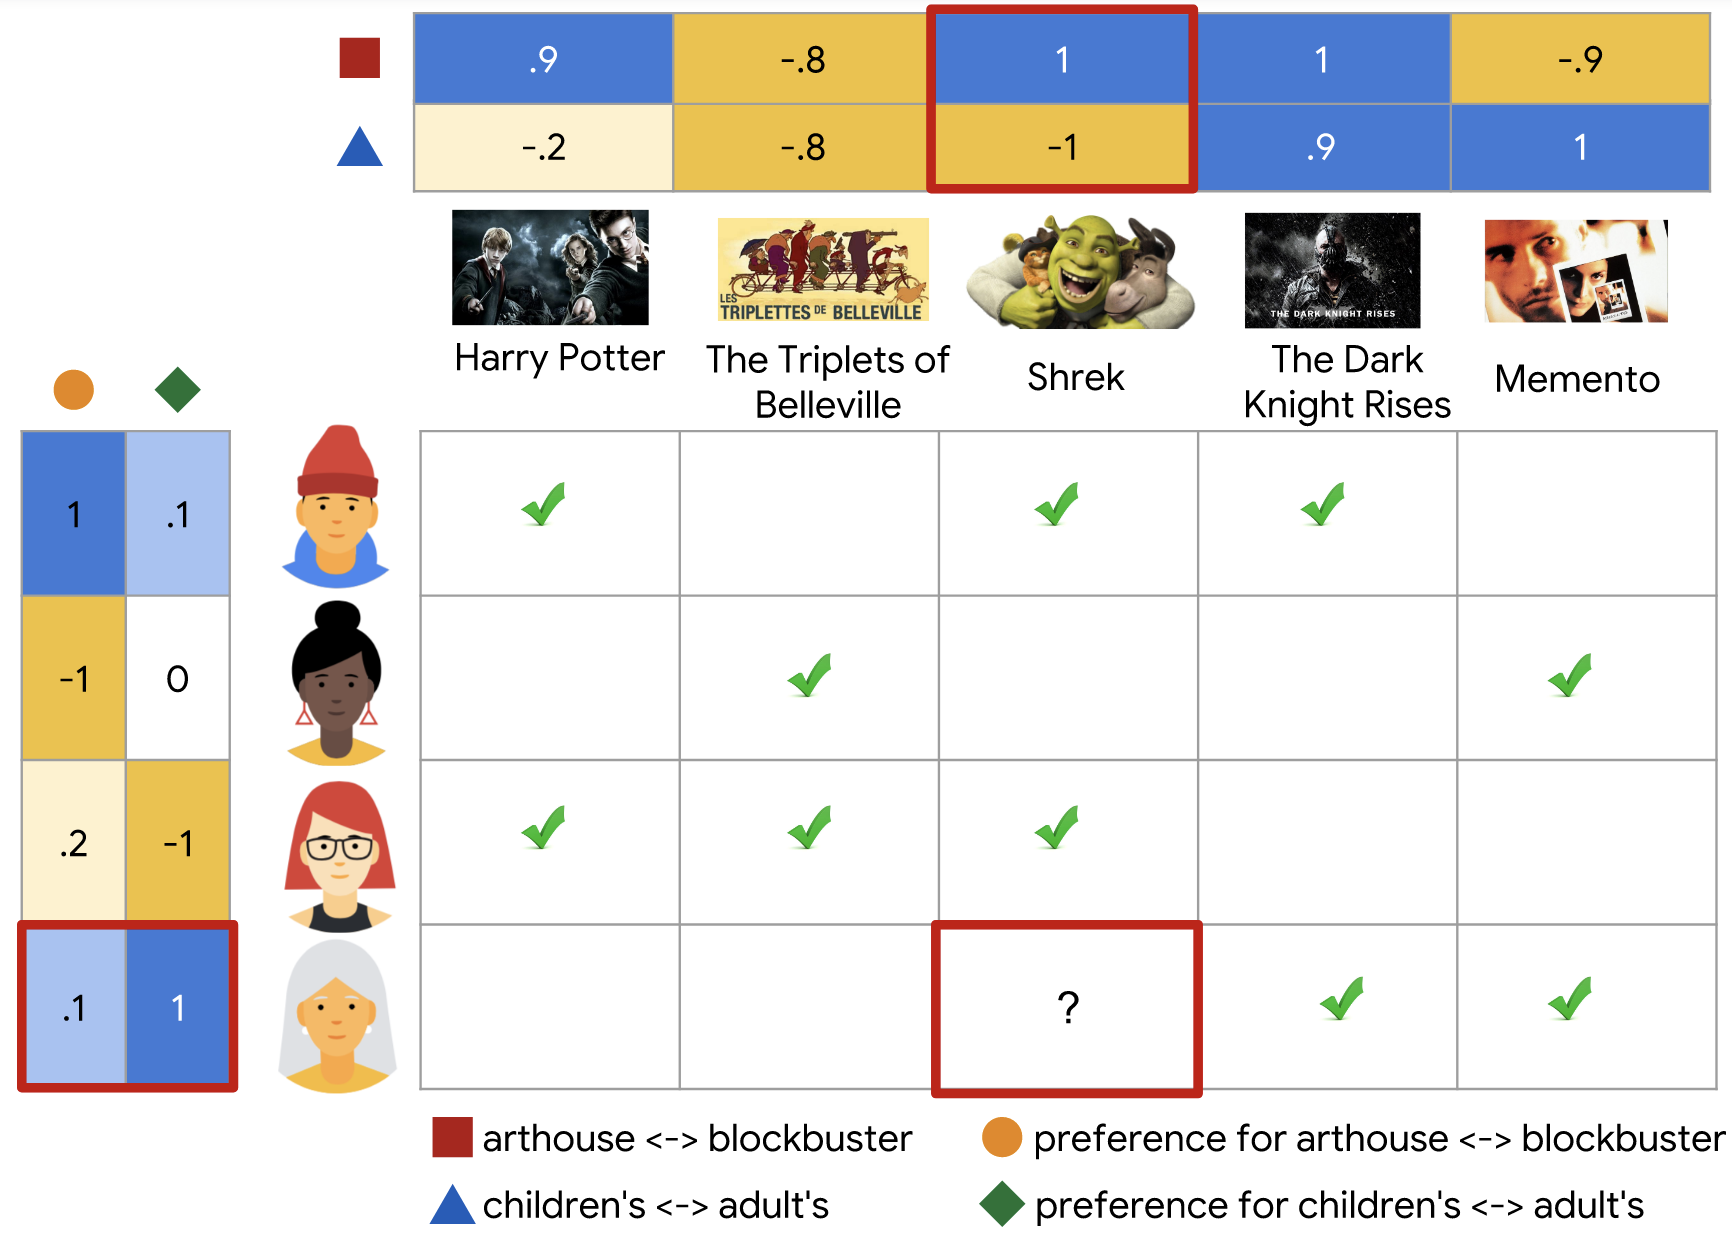
\includegraphics[scale=0.45]{images/latent_factors}
	\centering
	\caption{What latent factor values can tell us about user/item interactions \citep{httpsdevelopersgooglecom_matrix_2023}} 
	\label{fig:figure}
\end{figure}

This is useful for a sparse matrix (when most user/item interactions are zero), because it shows information that the matrix alone does not.  One can see trends of preference within the latent factors. Because it reduces the dimensionality of a given matrix. Matrix factorisation also requires less processing power than methods that search through the raw matrix. 

There are different ways of factorising a matrix. An example of one is Singular Value Decomposition (SVD). Equation 2.6 shows this with $U$ and $V$ matrices for a given number of dimensions,  where M is the approximated matrix:

\begin{equation}
	M = U \sum V ^{T}
\end{equation}

Alternating Least Squares, is a computational safe way to calculate M. It works by alternating between estimating the U and V matrices until it reaches closely to the value of M. Stochastic gradient (another method for calculating M) repetitively uses random bits of data to approximate U and V \citep{koren_matrix_2009}. 

When the matrix is split up, the predicted rating can be calculated from the user and item feature vectors. 


Looking at the latent factors one can find  similar items using a cosine similarity. When working with sparse data, its favourable to use Alternating Least Squares because of its greater potential for parallelisation (working out calculations simultaneously) \citep{koren_matrix_2009}.

\subsection{Limitations}
Despite its popularity, Collaborative filtering has limitations as a recommendation method.

\textbf{Sparse Data - }Not every user has listened to every song. This means in data sets, having a sparsity of around 98-99 \% is very common \citep{celma_recommendation_2010}.

\textbf{Grey sheep - }This is when a user has a unique taste that is dissimilar to most other users, making it hard to stem recommendation's from. This is a common problem with datasets that are very sparse \citep{claypool_combining_1999}.

\textbf{Cold Start and Early Raters - } The term cold start refers to new items whilst early raters refers to new user \citep{avery_recommender_1997}. When there are new users or items, there is little data associated with them so it is challenging to come up with suitable recommendations based on either the user or item. 

\textbf{Popularity Bias - } Collaborative filtering does not take into account information about the item, only user interactions with it. This means that it has a bias towards popular items \citep{celma_recommendation_2010}.

\textbf{Feedback loops - } When users interact with items that are recommended through Collaborative Filtering, based on previous user item interactions, it strengthens the initial recommendations more and creates a loop \citep{sanchez-moreno_incorporating_2018}.

\section{Content Based Filtering}

Content Based Filtering works by looking at the characteristics of a given item and see if it matches the preference of the user. Recommendations stem from the given information about the item, not what other users interact with. Item's information is found and then is used to find similar items\citep{casey_content-based_2008}. Music recommendation systems stem from song information that aligns with the users taste \citep{aucouturier_music_2002, logan_music_2004}. 

Early uses of content based filtering were text based, because of its ease of information extraction, An example of this is the PRES system \citep{van_meteren_using_2000}. Machine learning has enabled extraction of information from complex formats like images or audio. Models like "Xception" have proven successful at extracting audio features from songs \citep{chollet_xception_2017, singh_robustness_2022}.

There has been a lot of research on extracting musical components from an audio file \citep{ribecky_multi-input_2021, zhao_musical_2022}. Recent developments have shown successful extractions of genre and structure with the MusicBERT Model \citep{zhu_musicbert_2021}. It's found that MIDI extraction from songs can aid to give better solutions for less popular songs, helping eliminate the cold start problem \citep{yadav_improved_2022}.

Content based filtering looks at how similar the attributes of each item is when finding recommendations. It's decision making doesn't use subjective factors, like user behaviour. An item is used as a vector made of its defined values of attributes, where the distance between other items can be found. Distance can be calculated using Euclidean, Manhattan, Chebyshev, cosine distance and Mahalanobis distance. With two feature vectors equalling $x$ and $y$, equations are found below.
\\
\\
\textbf{Euclidean Distance:} The distance between two points.
\begin{equation}
	d(x,y) = \sqrt{\sum _{i=1} ^{n}(x_{i} - y_{i})^{2}}
\end{equation}

\textbf{Manhattan Distance:} The sum of the absolute differences between two vectors.
\begin{equation}
	d(x,y) = \sum _{i=1} ^{n} | x_{i} - y_{i} |
\end{equation}

\textbf{Chebychev Distance:} The greatest difference between two vectors.
\begin{equation}
	d(x,y) = man_{i} = _{1 . . n} | x_{i} - y_{i} |
\end{equation}

\textbf{Mahalanobis Distance:} The distance between a point and a distribution of points.
\begin{equation}
	d(x,y) = \sqrt{ ( x - y )^{ T } S^{ -1 } ( x - y ) }
\end{equation}

Euclidean, Manhattan and Chebychev distance are used when there is little relationship or correlation between attributes. If there is correlation, its advised to use Mahalanobis distance \citep{celma_recommendation_2010}.

Equation 2.11 is a delta function ($\delta $) and is used when attributes aren't measured numerically. When two attributes match it equals zero, other wise it equals 1.

\begin{equation}
	d(x,y) = \omega \sum _{ i = 1 } ^{ n } \delta (x _{i}, y _{i})
\end{equation}

Content based filtering overcomes the problems collaborative filtering has of being able to rate items that previously haven't had any ratings. Its also able to adapt to any changes in the users preference quickly \citep{isinkaye_recommendation_2015}. For users who don't want to share their data they can get suitable recommendations as well \citep{k_you_2006}.

\subsection{Limitations}
The cold start and grey sheep problem also occur in content based filtering. Popular items usually have better defined features, and older users have better represented features.

\textbf{Novelty Problem - } This is when the user is recommended items too similar to the one they already have, an application would need some way of diversifying recommendations to overcome this \citep{celma_recommendation_2010}.

\textbf{Retrieving metadata - } Despite recent improvements in extracting musical information \citep{vall_feature-combination_2019, singh_novel_2022}. This data is used in mainly in deep neural networks or hybrid models. Obtaining rich enough meta data to rely on Content Based Filtering alone is still not reliable.

\textbf{Suggestions not opinionated- } It doesn't take into the account the opinions of users, only description of what the item is. This may lead to some poor quality recommendations that only relying on observing features would obtain \citep{celma_recommendation_2010}.  

\section{Clustering}

Another method of finding similar items is Clustering. Clustering is when one  groups a collection of data objects, so that some objects clustered together are very similar, while other clustered objects are not alike. Similarity is then evaluated based on chosen parameters \citep{ferretti_clustering_2018}. A popular algorithm is the k-mean cluster where each cluster is representerd by a mean value of the object \citep{han_data_2006}. A model that uses an altered version of k clustering limits the randomness in the suggestion this method generates \citep{chang_personalized_2017}.


\section{Diversity issue}

Recommendation systems are used extensively by the majority of Spotify users \citep{spotify_spotify_2020}. However, there are a subsection of users who, despite huge breakthroughs, don't rely on algorithmic means of discovering music. In 2020, a study done found that users with more diverse tastes would find music in non algorithmic ways \citep{anderson_algorithmic_2020}. Users with less diverse taste relied on algorithms for recommendations. Users who's taste became more diverse, occurred from non algorithmic ways of finding music.

A reason for this is the small amount of listeners who have a diverse taste, lots of music recommendation systems don't focus on a specific type of person when training a model \citep{laplante_improving_2014}.

It's argued that the way classification is handled in music could also be a reason \citep{porcaro_diversity_2021}. The classification of music is a debate that has been passed from generations \citep{moles_sociodynamique_2019, dimaggio_classification_1987, bourdieu_distinction_2010}. In the context of a recommendation system, a genre being treated as a "tag" usually pushes its social and cultural relevance to the side \citep{porcaro_diversity_2021}. The act of a machine understanding a concept as subjective as genre is one that has proven challenging \citep{nurnberger_survey_2014}. Vlegels attempts to overcome this by organise groupings based on user artist relationship, rather than an artists genre \citep{vlegels_music_2017}.

This problem existing could be a reason for the continued need for "curation", the act of having a professional spot interesting things and document them to consumers \citep{barna_perfect_2017}. With this comes the role of a DJ, whom before recommendation systems existed, were doing just that \citep{percival_music_2011}. 

Recently there has been attempts of integrating DJs in streaming services.  An example of DJ's and algorithmic centric streaming apps coexisting is Apple Music's Beats 1 Radio station. The subscription service allows access to a radio station of the most popular artist and DJs in the western world broadcasting shows, providing entertaining commentary and selected musical recommendations \citep{dms_apple_2020}. Another is Spotify's curated playlists, and more specifically there track ID's series, where they get established DJs to make a huge ever changing playlist of songs they play out live \citep{spotify_introducing_2020}.  Seeing this type of content shows how a company can pedal a term like "curation" in the music world and see it as a necessity \citep{barna_perfect_2017}. One can see this in the rise of internet radio as well.  

Internet radio is a strangely thriving industry which is expected to have an net worth of \$9.2 Billion by 2030 \citep{market_research_future_internet_2022}. This boom has seen growth within DJ centric radio stations \citep{gillett_how_2021}. Its popularity can be drawn from increased speeds in mobile data, and choice of stations, but one can see that curation is a big draw to its appeal \citep{nts_2023}.

Despite the vast amount of data surrounding DJ sets, there's been little research on using DJ sets to train algorithmic models. A unique instance of this is found in Chows recommendation system made out of the many DJ mixes found on MixesDB. The application inputs a single song and outputs similar songs found through the dataset \citep{chow_music_2020}. Finding recommendations from multiple songs or another DJ set is something that has been previously unexplored, and could provide with solutions with assuring a exciting level of diversity that is missed in many recommendation systems.


\section{Summary}
The theory behinds recommendation systems were introduced and explained, with examples of current day models that use them. With its success, it was addressed from a survey that recommendation systems aren't commonly used with users with "diverse" music taste. The continued use of internet radio, DJ sets and curated playlists affirmed the findings of this survey. It was concluded that little research has been done on training an algorithmic model from DJ sets, potentially providing a recommendation system that would appeal to listeners with diverse taste. 

% note that \Blindocument has 5 numbered levels, despite setting secnumdepth above. I (and many style guides) would suggest using no more than 3 numbered levels (incl. the chapter), with the option of a fourth unnumbered level.

% Chapter 3
% !TEX root = ../TechProject.tex

\graphicspath{{Chapter3/}}

\chapter{Machine Learning used for DJing}

\begin{figure}[H]
	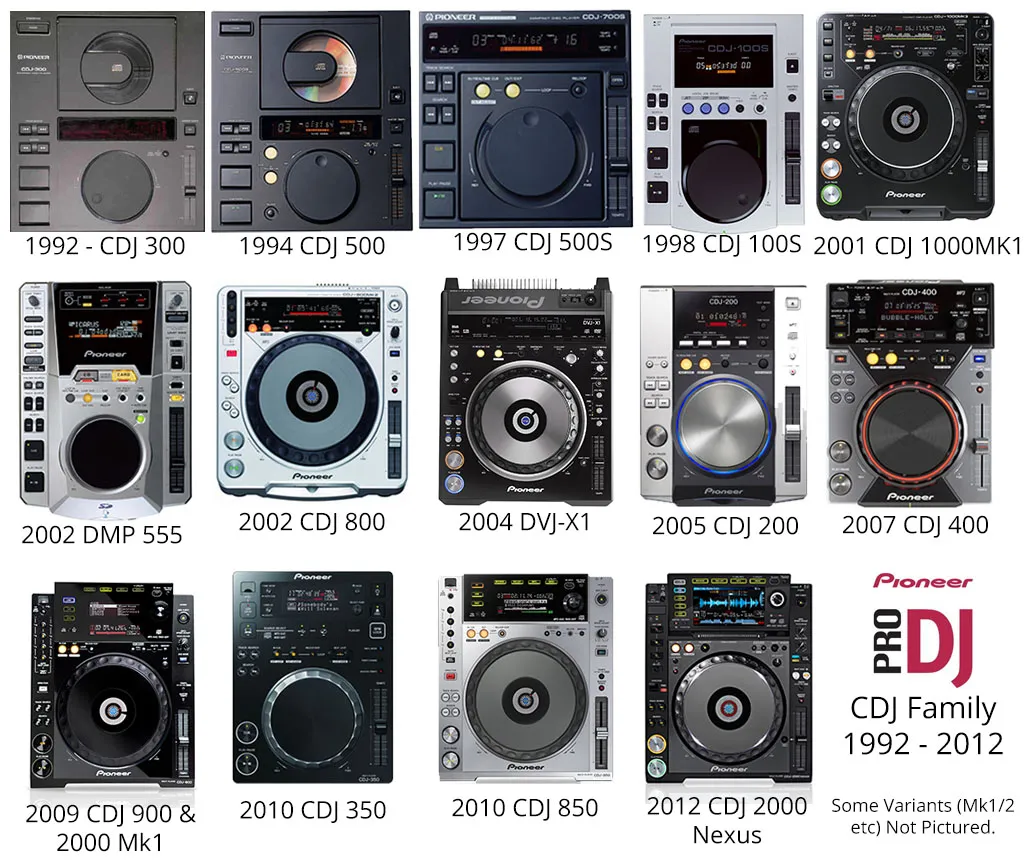
\includegraphics[scale=0.3]{images/pioneers_history}
	\centering
	\caption{Pioneer CDJ models from 1992-2012 \citep{chesters_history_2017}} 
\end{figure}

This chapter answers the following research question:
\\

\textit{Can a DJ-set centric dataset be used to solve other DJ tasks?} 
\\
\\
DJing (abbreviation of Disc Jockey) is a practice that has been the backbone of many sub cultures since the late 60s \citep{brewster_last_2014}. DJing has contributed to the evolution of various genres like Disco, Reggae, and the many forms of electronic dance music \citep{partridge_dub_2010, reynolds_energy_2013}. DJing traditionally involves two turntables and transitioning from one song to another in a stylised or fluid manner. The rise of digital audio during the 1990s saw the creation of CDJ's, and with it the introduction of mixing tool softwares such as Pioneer's rekordbox. Mixing tool software's makes use of music information retrieval techniques to lower the difficulty of organising and preparing for a DJ set \citep{kim_automatic_2017}. 

Music Information Retrieval is based on finding and compartmentalising the various aspects of music, including rhythm, timbre and melody \citep{orio_music_2006}. Implementations of music information retrieval vary from source separation and beat tracking. These tasks involve machine learning and deep learning algorithms, and are now fully embedded in DJ software \citep{rekordbox_rekordbox_2020}. 

\section{Source Separation}

Source separation involves estimating specific sources in one mixed signal \citep{jansson_singing_2017}. A music based example involves separating an instrument or voice within a track \citep{sgouros_efficient_2022}. Deep learning advancements have helped improve source separation in different fields. An example of this is U-nets, a convolutional neural network that proved effective in segmenting biomedical images \citep{ronneberger_u-net_2015}. With the use of spectrograms, a very similar model was used in a music source separation model \citep{jansson_singing_2017}. Deezer  further adapted this in their popular open source separator Spleeter \citep{hennequin_spleeter_2020}. Despite no published method, popular DJ manufacturer, Serato, released the Serato Stems update to there DJ software which provides similar functionality to Spleeter but in real time \citep{kirn_review_2023}. This has allowed DJs to make remixes in real time, separating instruments or voices from chosen songs.

As with most machine learning models, a rich dataset is essential for an application's accuracy \citep{jain_overview_2020}. The data used to trained for Jansson's U-Net model involved 20,000 track pairs of acapella and instrumental tracks \citep{jansson_singing_2017}. Isolated acapella or instrumental tracks are uncommon in DJ sets so the proposed model could not aid to further developments in source separation.


\section{BPM, key, genre classification}

\begin{figure}[H]
	
	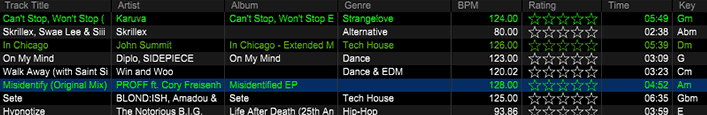
\includegraphics[scale=0.64]{images/rekordbox}
	\centering
	\caption{Playlist in rekordbox showing calculated BPM's and keys \citep{rekordbox_rekordbox_2023}} 
\end{figure}


Audio classification involves retrieving metadata from analysing an audio file \citep{sharma_audio_2021}. Audio classification models is used in DJ software's for calculating tempo, key and other musical attributes.

Despite increased popularity with deep learning, traditional machine learning techniques proves powerful enough for key detection. The Support Vector Machine proposed by George et. al had an accuracy value of 91.49\% and performed better compared to previous papers \citep{george_development_2022}. Support Vector Machine works well due its use of the kernel track and being able to handle linearity and non-linearity in data effectively \citep{hofmann_support_2006}. Having key information is essential within DJing because assuring the keys either match or modulate functionally assures fluidity in the transition. 

With tempo detection, Temporal Convolutional Networks are used effectively \citep{bock_deconstruct_2020}. Temporal Convolutional Networks are a hierarchy of temporal convolutions which can perform accurate detection and segmentation \citep{lea_temporal_2017}. The model was first used for tempo detection in 2019 \citep{bock_multi-task_2019}. The main breakthrough was the application  calculating the up beat and down beat, and through exploring both, each tasks saw increased accuracy from learning from the other \citep{bock_multi-task_2019}. When revisited in 2020, it was found that incorporating an extra dilation rate to each layer of the model gave more accurate results. Knowing the tempo of a given song is one of the main draws of CDJs over vinyl turntables, so further developments in tempo detection will inevitably find itself implemented in DJ software.

As the case for the BPM and key, recent advancements in genre classification have also ocurred. The most recent signification is a model that extracts short-time fourier transform, pitch, timbre and modified non-negative matrix factorisation features from a given piece of audio. These extractions are then fed through a deep belief neural network and optimised with a Wale Integreated sea lion algorithm \citep{kumaraswamy_optimal_2022}. A deep belief network is a generative model that uses stacks of restrictive Boltzmann machines (RBM) in its architecture \citep{canuma_what_2022}. The whale integrated sea lion algorithm is a nature inspired meta-heuristic optimisation algorithm that is good for advanced searches \citep{mirjalili_whale_2016}. Advancements in genre classification would be helpful within the DJ world as it would help the organisation of playlists for a given DJ.

Due to the dataset being built from DJ sets, it's unrealistic that the proposed method could compete with the classification methods discussed. However, a dataset built from DJ set could show audio examples of inputted songs being mixed.

\section{Automated Mixing}
Advances in classification and separation can automate preparation tasks for a DJ. However, there has also been deep learning advances that could all together replace a DJ. In February 2023, Spotify unravelled its brand new DJ feature. It combined situational music recommending accompanied by an AI generated host, mimicking the role of a personal broadcast DJ \citep{naomi_spotify_2023}. Within the research world, there have been advances on not just the mimicking of a human DJ's dialogue, but also the way in which a human would transition from one song to the next \citep{chen_automatic_2022}.

Spotify have had DJ style transitions and have ran experiments to show a general further appreciation to playlist that includes them \citep{bittner_automatic_2017}. In Bittner's  attempts to model DJ-style tranistions, peak detection is used to determine where-bout's in the song the "drops" occurs. Specific rules are given to assure appropriate drop in and drop out points for a given track \citep{bittner_automatic_2017}.  However Spotify's means of working out up and down beat was ineffective and greatly effected the fluidity of the transitions. A recent attempt found that using Boykov-Kolmogorov algorithm alongside spectrogram analysis of the two given songs made for great results for songs with similar tempos and keys \citep{robinson_automated_2023}. These models work with datasets very similar to the one in the proposed model. A fader estimation investigation ran in 2022 even uses MixesDB as a training dataset \citep{kim_joint_2022}. This indicates that a DJ-set centric dataset could be used to estimate parameter values during transitions from a dataset of DJ sets and audio files of songs in the tracklist.

\section{Summary}
An overview of DJing was given and how advancements in music information retrieval has helped its evolution. The recent technology behind Source separation, classification and automatic mixing was discussed. It was concluded that if the proposed model was developed further,useful information in regards to transitions could be found.

% note that \Blindocument has 5 numbered levels, despite setting secnumdepth above. I (and many style guides) would suggest using no more than 3 numbered levels (incl. the chapter), with the option of a fourth unnumbered level.

% Chapter 4
% !TEX root = ../TechProject.tex

\graphicspath{{Chapter4/}}

\chapter{Hypothesis}

\section{Literature Review Conclusions}

The literature review set out to answer the two questions:
 
 \begin{enumerate}
 	\item \textit{What are effective methods for the automated recommendation of songs suitable for adding to a given DJ set?}
 	
 	\item \textit{Can a DJ-set centric dataset be used to solve other DJ tasks?}
	\end{enumerate}
 
 It was shown that the current machine learning advances in separation and classification could aid a DJ greatly, but despite great advances in recommendation systems, algorithmic ways of gathering song recommendations do not handle the cultural significance of genre and style.

With this being the case, modern day recommendation systems don't usually cater to the traits found in both professional and hobbiest DJs. Preparing a DJ set requires a sizeable amount of music \citep{allen_djs_2021}. Based on the research ran by Anderson, DJs would certainly fall in the category of diverse \citep{anderson_algorithmic_2020}.

The necessity to reach a certain quantity of songs to DJ, requires collecting or "digging" for songs. Digging is a pre digital era term, to go find music in specific record stores or from esoteric places, with the higher likelihood of picking up something that could be emotionally resonant \citep{allen_djs_2021}.

Recommendation systems could be seen as a replacement for digging. A given application should knows if a user wants esoteric music. But as mentioned in the Diversity Issue sub-section, finding these sorts of recommendations relies heavily on the cultural context surrounding a genre and with it gives less desirable suggestions compared to manually finding music. 

This problem is somewhat resolved with the popularity behind sites like Bandcamp, which prides itself with regularly updated blog posts, and the option to examine other people collections. These features encourages users to "dig" more so than other music based platforms \citep{bandcamp_about_2023}.  These sites can be a great resource to find music in a digging manner, but having an algorithm do it would be more time efficient. 

Successfully training a model from this type of dataset could then be used to algorithmically suggest quality songs, and potentially assist other DJ related tasks.

Aside from Daniel Chow's model, a recommendation system that attempts to mimic suggestions found from digging is yet to happen \citep{chow_music_2020}. Adapting modern day recommendation systems to this task gives lacklustre results.

\section{Algorithmic ways of obtaining recommendations from a DJ set}
\begin{enumerate}
	\item \textbf{Spotify }- Find a DJ set on Spotify, add that to a playlist, and look for the"
	Recommended based on the playlist" . The main problem with this is that DJ sets on Spotify are few and far between. Not many can be found, but labels like !K7 publish DJ sets commercially \citep{k7_about_2023}. The system also finds what other users are listening to, often giving song recommendations that are usually quite popular and well-known.
	
	\item \textbf{SoundCloud }- Many DJ sets are found here, and using the "radio" function, recommendations can be found. However, it prioritises other DJ sets on its "radio " rather than songs. The recommendation system is also only limited to what is available on SoundCloud.
	
\end{enumerate}

\section{Hypothesis proposal}
	
The hypothesis is that the application will give song recommendations that are both stylistically suitable but aren’t necessarily popular. Its common for a DJ, having a diverse taste, to go into
great lengths to find obscure and unknown songs. Therefore, not prioritising popularity is a
desirable trait in a recommendation system for a DJ’s music consumption and knowledge, usually
being more than the average consumer. Its a common trait in most music recommendation
systems to prioritise popularity. Building a recommendation system from a dataset of DJ sets
will hopefully give these types of suggestions.	

With DJ sets being the intended input of this model, one hopes that its accuracy is comparable with top performing recommendation system models.

\section{Summary}
The literature review was summarised and the gaps in research was stated. An overview of obtaining recommendations for a DJ set was given. A hypothesis given  hopes the accuracy of the model would be comparable to top performing model, when DJ sets are used as inputs. 



% note that \Blindocument has 5 numbered levels, despite setting secnumdepth above. I (and many style guides) would suggest using no more than 3 numbered levels (incl. the chapter), with the option of a fourth unnumbered level.

% Chapter 5
% !TEX root = ../TechProject.tex

\graphicspath{{Chapter5/}}



\chapter{Application}

Inspired by the training data from a fader estimation investigation, MixesDB is a website of archived DJ sets \citep{kim_automatic_2017}. With over 260,000 mixes on the site, using this as a dataset to train the model proved to be an excellent choice \citep{mixesdb_main_2023}.

The application is a two-stage Music Recommendation system trained on DJ sets found on MixesDB. First, a collaborative filtering algorithm, alternating least squares is used to gather initial suggestions. Then, the audio features the Spotify API provides will be used to create vectors to refine the selection further. The best songs are selected using euclidean distance to measure the distance between vectors. 

It was coded using a 2020 16GB MacBook Pro in \textit{Python}, and the following libraries were used:
\begin{itemize}
	\item \textit{pandas:} Used for managing the dataset.
	\item \textit{implicit:} Its alternating least squares function was used for the initial suggestions.
	\item \textit{spotipy:} Used to access audio features from the Spotify API.
	\item \textit{scipy:} Its euclidean distance function was used for the final suggestions.
	\item \textit{Pytest:} Used for unit-testing.
\end{itemize}

As mentioned in Chapter 2, Daniel Chow built a system that takes in a single song and outputs similar songs based on the MixesDB dataset \citep{chow_music_2020}. His code will provide the foundation extended by adding multiple inputs and an extra layer of recommendation filtering.

\section{Data set}
The data was scraped from MixesDB using Selenium \citep{chow_music_2020}. The tracks in a given DJ Set, which had a corresponding Spotify link, were stored with a given user ID for the DJ. In cases where a single DJ set included multiple DJs, the set was considered as belonging to all the DJs involved, and the corresponding songs were linked to each DJ's user ID. The data set only has DJ sets up to 2020, the year Daniel Chow wrote the article. The dataset has approximately 9900 DJ sets and 99100 songs. Figure 5.1 shows a DJ set from the dataset.
\begin{figure}[H]
	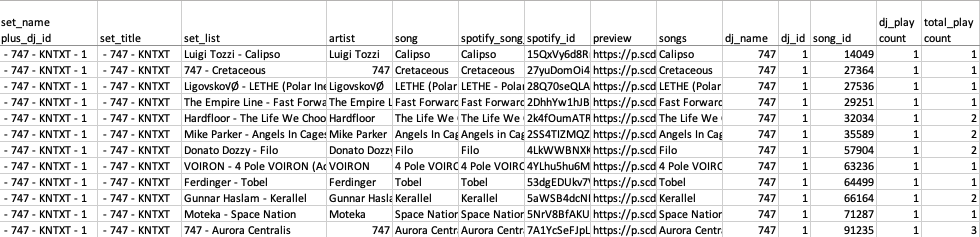
\includegraphics[scale=0.4]{images/dataset}
	\centering
	\caption{Table showing a DJ Set in the dataset} 
\end{figure}


\section{Initial Suggestions}
\begin{figure}[H]{\noindent\ignorespaces}
	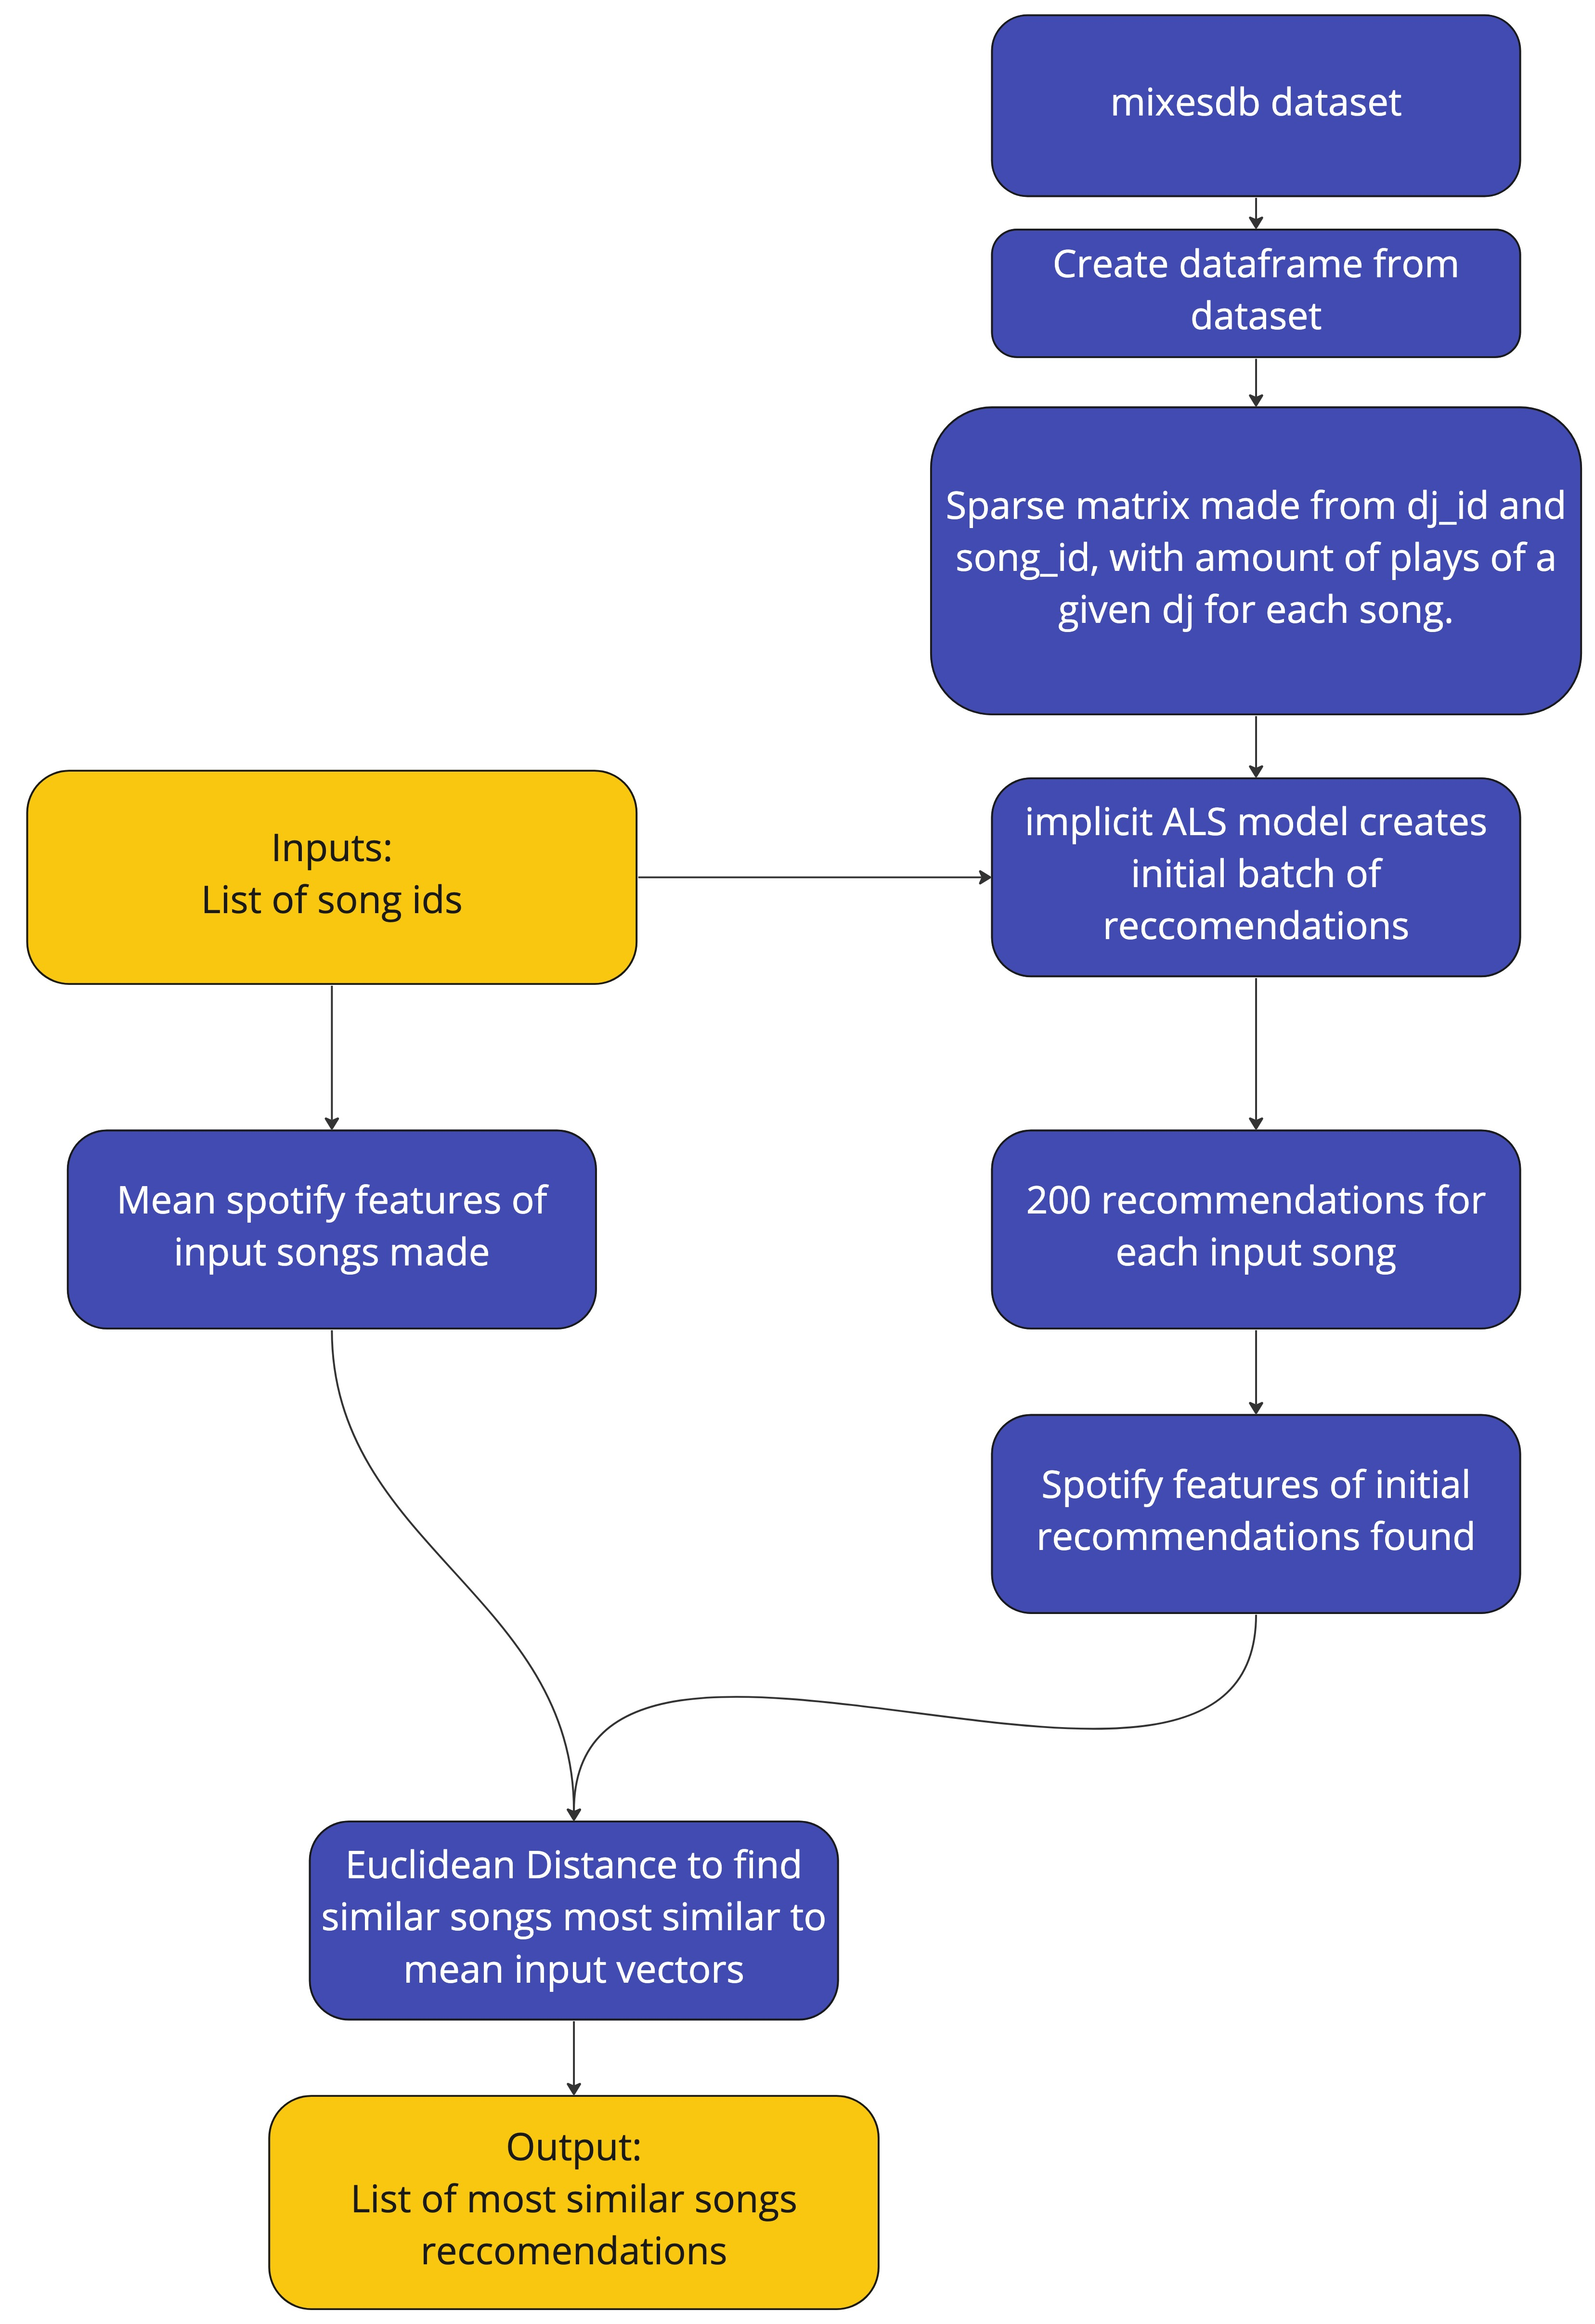
\includegraphics[scale=0.09]{images/application_app_flow}
	\centering
	\caption{A flow diagram of the application} 
\end{figure}
As in Daniel Chow's method, the initial suggestions part of the model is made using alternating least squares. The Netflix Prize award made this matrix factorisation algorithm popular \citep{zhou_large-scale_2008}. As explained in Chapter 2, this method is suitable for two reasons. It provides a computationally efficient way of handling a dataset and splits the DJ song matrix into its latent factors. The latent factor values reveal trends between songs and DJs.

A model is made from the dataset, and then the input list of songs is processed. Next, the alternating least squares algorithm is run for each song to find other similar songs. The number of recommended song suggestions for each song was set to 200 to ensure that many similar songs are used in the refinement stage.


\section{Final Suggestions}
To add an extra filtering layer, the Spotify API is used to explore further which songs are the most similar.

The Spotify API provides audio features for each song using both the input songs and initial suggestions. The features used are shown below \citep{spotify_web_2023}:

\begin{enumerate}
	\item \textbf{acousticness} - A measure of how acoustic the song sounds, the range is from 0 - 1, with 1 being definitely acoustic and 0 being not acoustic at all.
	\item \textbf{danceability} - Measurement of how suitable a track is for dancing based on tempo, rhythmic features and overall regularity. 1.0 is the most danceable. 
	\item \textbf{energy} - A measurement of intensity and activity. Typically, energetic tracks feel fast, loud, and noisy. A heavy metal track would score high, but a Bach prelude would score low. Attributes, including dynamic range, perceived loudness, timbre, onset rate, and general entropy, will dictate this value. 1.0 is highly energetic.
	\item \textbf{instrumentalness} - Predicts whether a track contains no spoken vocals. Songs scoring 1 likely have no vocals. Values above 0.5 represent instrumental tracks.
	\item \textbf{key} - The tracks key uses the following notation 0 = C, 1 = C$\sharp$/D$\flat$, 2 = D. If the key cannot be detected, then the value is set to -1.
	\item \textbf{loudness} - Loudness of a given track in dB.
	\item \textbf{tempo} - The beats per minute of a given track.
	\item \textbf{time\_signature} - Time signature with the following notation, 3 = 3/4, 4= 4/4, 5 = 5/4.
	\item \textbf{speechiness} - Detects if a song has spoken word, audiobooks would score 1 and values ranging from 0.3-0.6 would be a combination of music and speech.
	\item \textbf{valence} - A measurement of how happy-sounding a song is. With scores of 1 being extremely positive.
	
\end{enumerate}

These features provided great data to form vectors for each song, as they highlight attributes of a song which makes them unique. Attributes like tempo are beneficial for improving the recommendations for DJ sets due to being the controlled variable when transitioning from one song to another.

As the input contains many songs, multiple steps are required to calculate euclidean distance. A mean vector is created from all the input song vectors. The vectors are then scaled. This step is crucial because some attributes work with different ranges, such as loudness using the dB range and acousticness from 0-1.

Once these are found, the euclidean distance between each initially suggested song vector and the average input vector is calculated. As discussed in chapter 2, euclidean distance is a way of measuring the distance between two vectors. An equation is shown at 5.1, allowing $x_{i}$ and $y_{i}$ to be two song vectors.

\begin{equation}
	d(x,y) = \sqrt{\sum _{i=1} ^{n}(x_{i} - y_{i})^{2}}
\end{equation}

For finding the vectors with the smallest distance between the mean input, this clearly represents that a given song has similar Spotify feature attributes. Therefore would be a worthy suggestion based on the recommended songs.

\section{Example Findings}
To spot-check the application in a non-methodical way, various DJ Set tracklists corresponding to different genres were used as inputs. Three different DJ sets were used:

\begin{itemize}
	\item \textbf{Rory Bowens, PLO Man, C3D-E, Brian Not Brian - The Slip, NTS Radio: } 
	\begin{itemize}
		\item \textbf{Genre:} New wave \& House
		\item \textbf{Tracks available:} 3/21
	\end{itemize}
	\item \textbf{Moxie, Shanti Celeste, Chris Farrell - NTS Radio: } 
	\begin{itemize}
		\item \textbf{Genre:} Tech-House
		\item \textbf{Tracks available:} 10/28
	\end{itemize}
	\item \textbf{Chimpo b2b L U C Y @ Keep Hush Live: Sherelle Presents:}
	\begin{itemize}
		\item \textbf{Genre:} Jungle \& Breaks
		\item \textbf{Tracks available:} 8/21
	\end{itemize}
	
\end{itemize}


When going through the recommended songs, the BPMs of the output songs were observed to see if they were around the same range as the input songs. The songs were listened to see if stylistically they were similar to the input songs, and the source of the recommended songs was also observed.

\begin{itemize}
	\item The Slip set performed okay. Expectations were low due to the small number of tracks available. Two input songs had a House style, and one was Indie. The recommended songs were all House songs, and none matched stylistically to the one indie song. However, all the BPMs were in a similar range around 110-120 BPM.
	\item The Moxie set performed very well. The input songs were all Tech-House songs, and the output songs were that as well, with a couple of more disco-inspired tunes. BPMs were all very similar as well.  
	\item The Keep Hush set also gave good results. The BPM ranges were similar to the input songs and stylistically matched the input songs well. 
\end{itemize}

All the suggested tunes did not come from an eclectic mix of DJ Sets or DJs. In each batch of suggestions, many songs were either from the same mix or the same DJ. 

The spot-checking intended to show the application in action rather than to dissect the quality of its performance, which is analysed in the Experiment chapter. A table of the input and recommended songs for the Moxie DJ set is shown in the table below.
\\
\\
\\
\begin{center}
	\begin{tabular}{ |c|} 
		\hline
		\textbf{Moxie, Shanti Celeste, Chris Farrell - NTS Radio}\\ 
		\hline \textbf{Input Songs}\\ 
		\hline Escape Earth \textit{Gravity Well} \\ 
		\hline Priori \textit{6thematic }\\
		\hline Carter Bros. \textit{Run - Monty's Bonus Beats}\\
		\hline Tyler Dancer \textit{Karmán Line}\\ 
		\hline Anunaku \textit{Forgotton Tales}\\
		\hline Piezo \textit{Tinned}\\
		\hline KMA Production \textit{Cape Fear}\\
		\hline Parris \textit{Dusty Glass Bubbles}\\
		\hline Tornado Wallace \textit{Open Door - Born Inna Tent Mix}\\
		\hline Luke Slater \textit{I Want You Too}\\
		\hline \textbf{Recommended Songs}\\ 
		\hline Black Booby \textit{Fill My Cup}\\
		\hline Omar S, John FM \textit{Heard'chew Single}\\
		\hline Hammer \textit{Manaka}\\
		\hline Awanto 3 \textit{Pregnant}\\
		\hline Steve Murphy \textit{Next Saturday - Club Mix}\\
		\hline Chasindub \textit{Still Here}\\
		\hline Ian Pooley \textit{Swing Mode}\\
		\hline Hashin \textit{Al-Naafyish (The Soul) - The "It's" About "Time" Remix}\\
		\hline Synkro \textit{Look at Yourself}\\
		\hline Kapote \textit{Uhh Baby - Brame \& Hamo Remix}\\
		\hline
	\end{tabular}
\end{center}


\section{Summary}
An overview of the proposed application was given. The first part described the alternating least squares method borrowed from Daniel Chow's model. Then the audio features found through the Spotify API were explained, and how it was used to form vectors. These vectors were then used to filter through the recommendations further. Finally, spot checking was done, showing suitable recommendations.




% Chapter 6
% !TEX root = ../TechProject.tex

\graphicspath{{Chapter5/}}


\chapter{Experiment}


As explained in the hypothesis, a music recommendation system that uses MixesDB as a dataset was made. An experiment was run to see if it garners appropriate results and will help answer the following question:
\\
\\
\textit{Is the proposed method a suitable solution to automate recommendations of songs suitable for adding to a given DJ set?}.
\\

R-Precision is often used as a performance metric to evaluate the quality of a recommendation system. 

\section{R-Precision}

\begin{equation}
	R-Precision = \frac{|G\cap R_{1:|G|}|}{|G|}
\end{equation}
R-precision is the number of found tracks originally in the mix divided by the number of known missing tracks. This is shown in the equation in 6.1, allowing $G$ to be the set of missing songs and $R$ to be the set of recommended songs.

R-Precision was used in the 2018 Recsys Convention idea for testing submissions for the million playlist challenge dataset from Spotify \citep{aicrowd_aicrowd_2023}. Competing teams built a recommendation system trained with the Spotify dataset at this convention. To test its quality, a challenge dataset containing many modified playlists was used to test the models.

It is essential to note the considerable difference in the number of DJ sets/playlists between the MixesDB and the Spotify dataset. The MixesDB dataset contains over 9800 DJ sets, while the Spotify dataset contains 1,000,000 playlists. The differences between playlists and DJ sets are worth mentioning as well. A playlist is a collection of songs, regardless of cohesion or song count, while a DJ set is typically a seamless mix of songs that can vary in length from 8 hours to no less than 20 minutes.

The top 10 scoring models from the convention have R-Precision values ranging from 0.21 to 0.22. Given the differences in dataset size and task, aiming for an average R-Precision value of 0.171, slightly lower than the top-performing models, would be appropriate. Achieving this value would rank the model within the top 30 models trained by members of the public on the given Spotify dataset \citep{aicrowd_aicrowd_2023}. This approach allows for a fair comparison between the different systems and considers the unique characteristics of the dataset and task at hand. 

As the dataset utilised with the proposed model was obtained from MixesDB, a customised approach for preparing the evaluation set was conducted.

\section{Preparing Evaluation Set}
During the evaluation phase of the million playlist challenge, the quality of given applications trained on this dataset was assessed through various methods that involved analysing missing and recommended songs. In order to effectively compare different applications, it was essential to create a standardised evaluation set that incorporated aspects of the Spotify data set to show if a submitted application could recommend songs featured in the original playlist.

\begin{figure}[H]
	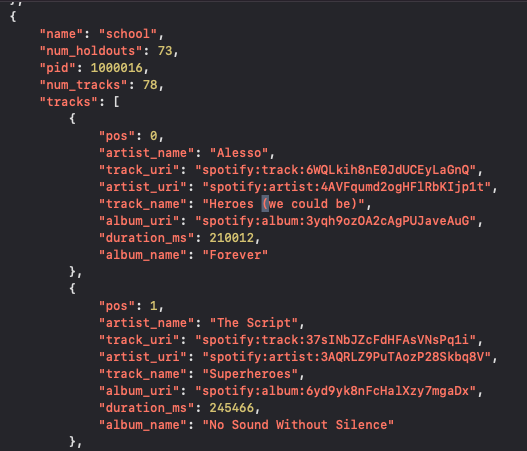
\includegraphics[scale=0.5]{images/spotify_challenge_set}
	\centering
	\caption{Screenshot of Spotify challenge set. \citep{aicrowd_aicrowd_2023}} 
\end{figure}

The Spotify challenge set consisted of 10,000 playlists with varying numbers of input songs, ranging from 0 to 100 tracks. For each of these playlists, Spotify requested 500 track recommendations from the participating teams \citep{aicrowd_aicrowd_2023}. However, due to the smaller dataset scale and the difference between playlists and DJ sets under consideration, various aspects of the challenge set used on the proposed model had to be downscaled. For instance, the range of input songs was considerably narrower, as DJ sets typically have a minimum length of 10 tracks, compared to playlists that can have varying lengths.
\\
\\
To ensure all songs in the evaluation set could be found, each song had to have a total play count of at least 5. This means each song had to be played 5 times by other DJs within the training set. This value was chosen to ensure that each song in the set would likely be found in the training set. Furthermore, the input and missing songs were split in the following way, with 20\% of the songs allocated as missing songs and the remaining 80\% as input songs. This was done to ensure enough songs were inputted. The output value for the application was also changed from 10 to 100 to better match the output for the evaluation given for the \textit{Spotify} dataset.

The making of the evaluation set was coded in \textit{Python} using the \textit{pandas} library, and \textit{pytest} was used for unit-testing.
\\
\\
\begin{figure}[H]
	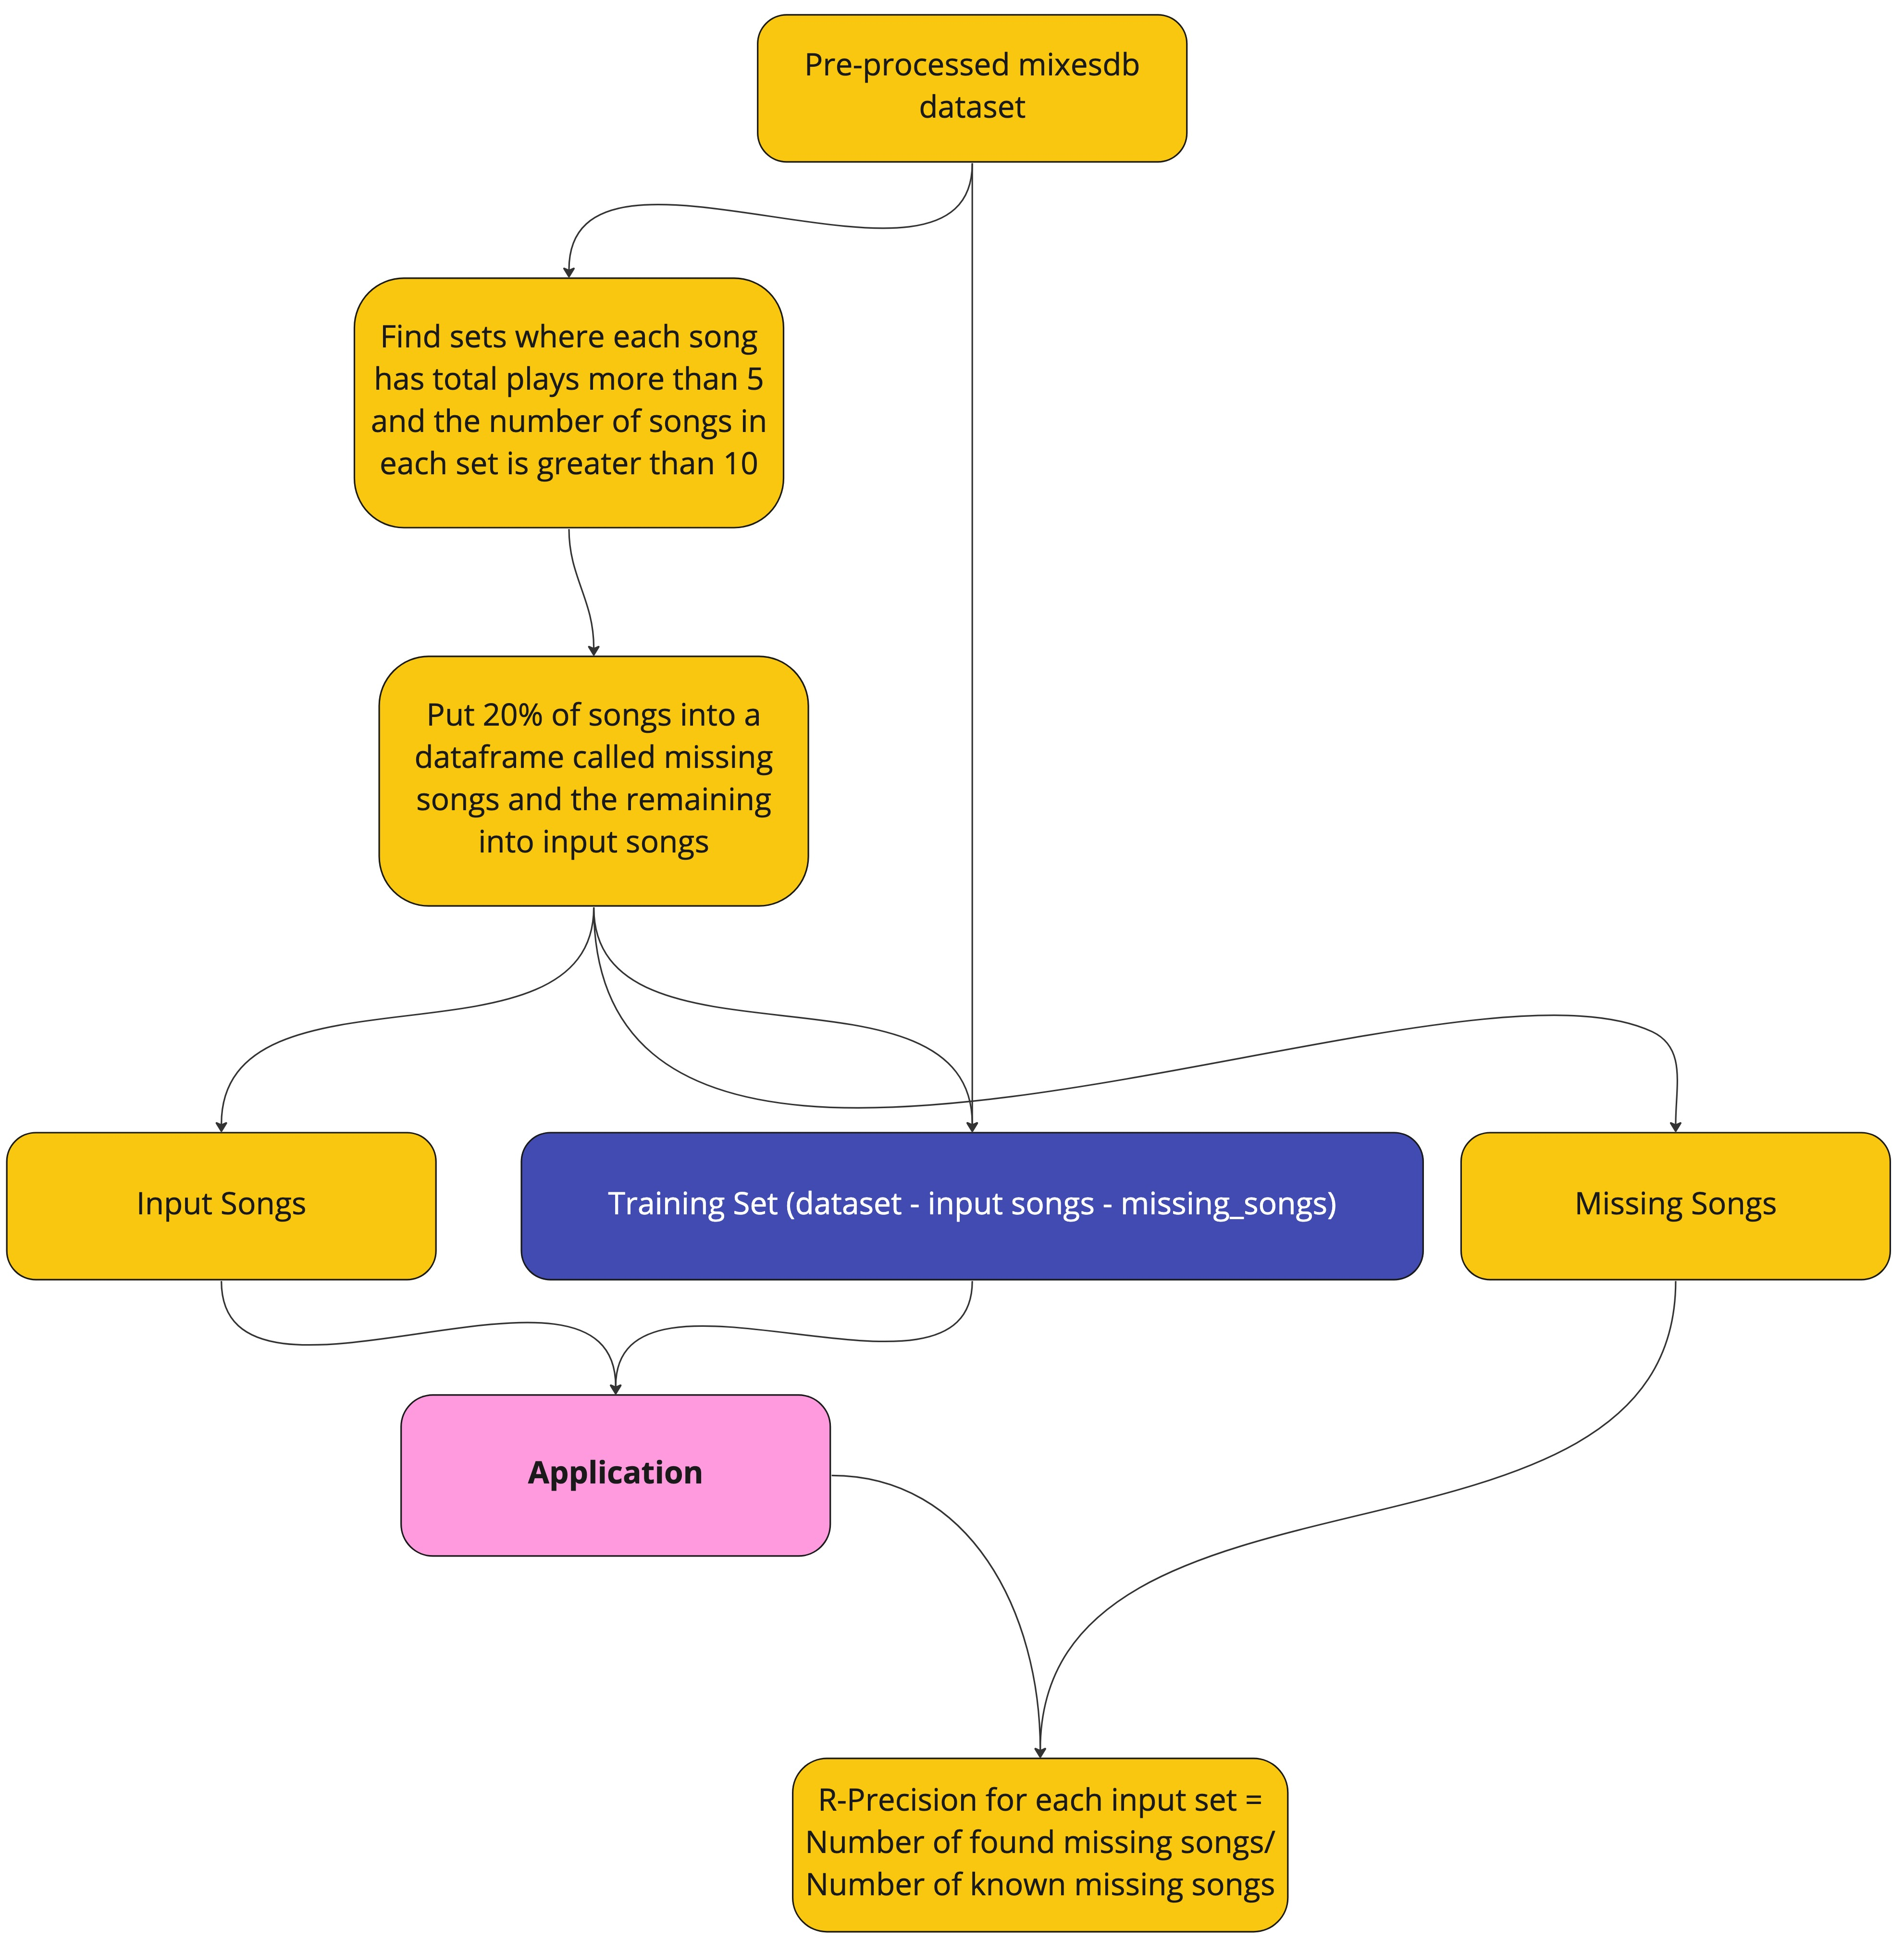
\includegraphics[scale=0.1]{images/evaluation_set_app_flow}
	\centering
	\caption{Application flow of the creation of the evaluation set} 
\end{figure}
\break
\section{Experiment Variables}

As mentioned in chapter 5, the proposed application utilises the alternating least squares algorithm to generate an initial set of suggestions. This algorithm is based on matrix factorisation, where the latent factors are derived from the training dataset to identify similar songs. Selecting an appropriate value for latent factors is crucial in ensuring the optimal performance of the algorithm. A low latent factor value may yield random results, while a too high value may lead to over-fitting \citep{zhou_large-scale_2008}. To identify the ideal value for latent factors, it is necessary to conduct an investigation where the latent factors will be the independent variable, and the average R-precision value will be the dependent variable. 

Once the best R-precision value is obtained, an examination of how changes to the size of the input DJ sets, impact the R-Precision value. From there, the R-precision value is compared to the highest-performing recommendation systems that use the Spotify dataset to see if the DJ-set-focused recommender can compare to industry standard models.

The experiment was run on a 16GB 2020 MacBook Pro.

\section{Summary}
An overview of the Spotify challenge set was given. The changes that had to be made to create a challenge set out of the MixesDB dataset were explained. It was shown how the evaluation set was made. 

The description of the test plan was shown. The initial independent variable was latent factors, then the input DJ set size. The experiment will be concluded by comparing r-precision scores with top-performing models trained on the Spotify dataset.



% Chapter 7
% !TEX root = ../TechProject.tex

\graphicspath{{Chapter6/}}

\chapter{Results and Discussion}

This chapter provides analysis and discussion of the results from the experiment described
in Chapter 6. The experiment sought to answer the question presented in Chapter 5.
\\
\\
\textit{Is the proposed method a suitable solution to automate recommendations of songs suitable for adding to a given DJ set?}.
\\

Chapter 7.1 will present the appropriate latent factors to use on the dataset. Chapter 7.2 explores if varying the input DJ Set tracklist lengths could also improve the models R-Precision value.

\section{Latent Factors}
The controlled variable is the list of input DJ sets and the independent variable was the number of latent factors for the alternating least squares part of the model. In the medium article, Chow used 50 latent factors \citep{chow_music_2020}. This was used as a reference point to make the range from 20 - 110 latent factors to experiment on. R-precision is the dependant variable.

Figure 7.1 shows a scatter graph of the average R-precision over different latent factors. The analysis shows that the performance of the application varies significantly with the number of latent factors used. The highest average r-precision of 0.1207 was obtained when 80 latent factors were used, while the lowest value of 0.0774 was obtained when only 20 latent factors were used. However, the performance of the algorithm was not monotonically increasing or decreasing with the number of latent factors. For instance, there was a slight increase in average r-precision from 40 to 70 latent factors, but a decrease from 50 to 60 latent factors. From 90 to 100 we see a significant decrease in the average r-value, which suggests that over-fitting is occurring.

\begin{figure}[H]
	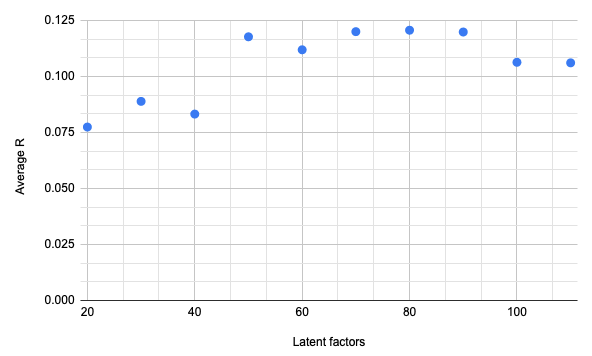
\includegraphics[scale=0.6]{images/average_r_over_latent}
	\centering
	\caption{Scatter graph of average r-precision values with different latent factors} 
\end{figure}

It's evident too few latent factors and too many latent factors affect the performance of the model. Therefore, it is important to strike a balance between the number of latent factors and the algorithm's performance.

\section{Varying input set length}
Given that an optimal latent factor value of 80 was determined, it is worth seeing if r-precision changes with the number of input songs in a DJ set. Increasing the the input set size could potentially improve the models accuracy, due to having more missing songs to pick from. The independent variable in this section is the evaluation set parameters and the dependent variable is the average r-precision value.

In Figure 7	.2, a scatter graph illustrates the r-precision values of each DJ set when the number of latent factors was set to 80. The graph reveals that the majority of the sets scored a value of zero, indicating that the recommendation system did not perform well for these sets. The highest score observed was 0.8, which suggests that the system provided a reasonably accurate recommendation for that particular set.

However, as the number of input songs in the DJ sets increased beyond 30, there was relatively fewer results available, but none of the DJ sets had an r-precision value of zero. This finding suggests that the recommendation system improved in its ability to provide accurate recommendations for sets with a larger number of input songs.

\begin{figure}[H]
	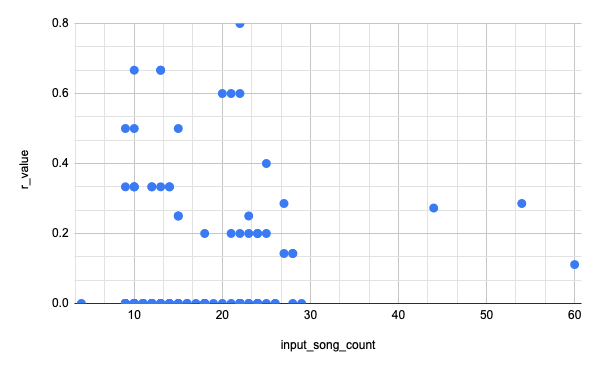
\includegraphics[scale=0.6]{images/80_little_sets}
	\centering
	\caption{Scatter graph of r-precision values with latent factors as 80} 
\end{figure}


When observing the changes in latent factors, the evaluation set was pulling from DJ sets that had 10 songs or more, and to include sets where each song has a total play count greater than 5. To  focus in on larger DJ sets, the total play count was lowered to 2 and then filtering on just DJ sets with over 20 songs.

Figure 7.3 shows the impact of input set size change on r-precision values, still using a latent factor value of 80. The results reveals  that the majority of DJ sets still had an r-precision value of zero. The highest r-precision value observed in this scenario was 0.6, and the average r-precision value was measured at 0.0865, suggesting that the application does not achieve higher levels of accuracy with an increase in input set size. These findings highlight the limited impact of larger input sets on the overall performance of the model.

\begin{figure}[H]
	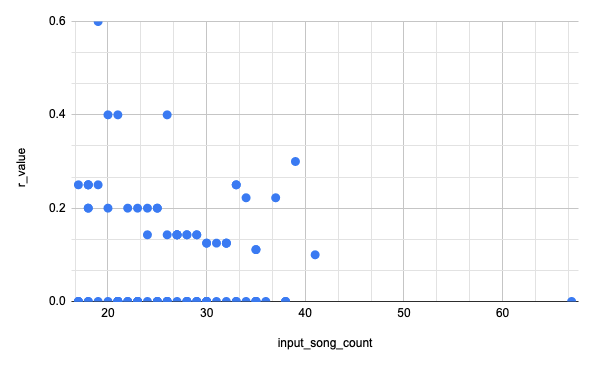
\includegraphics[scale=0.6]{images/80_big_sets}
	\centering
	\caption{Scatter graph of r-precision values with latent factors as 80 pulling from larger DJ sets} 
\end{figure}


\section{Comparing with industry standard models}

	The concept of calculating an R-precision value was introduced in the RecSys 2018 Spotify playlist dataset, where participants were tasked with building music recommendation systems for a given playlist. Normalised Discounted Cumulative Gain and Recommended Song Clicks were also used to measure the applications quality. Figure 7.4 illustrates the highest-performing teams in the said convention. The maximum average value attained by the application in question was 0.1207, which is significantly lower compared to the top 10 values. The dataset and challenge was eventually made open to the public, and compared to the results found on the leader-board, the application would have ranked 46th. 

It's low ranking suggests that the proposed method is not a suitable solution for finding valid recommendations for a given DJ set, due to the low average r-precision value when a collection of DJ sets were inputted.
\begin{figure}[H]
	\hspace*{-0.5cm} 
	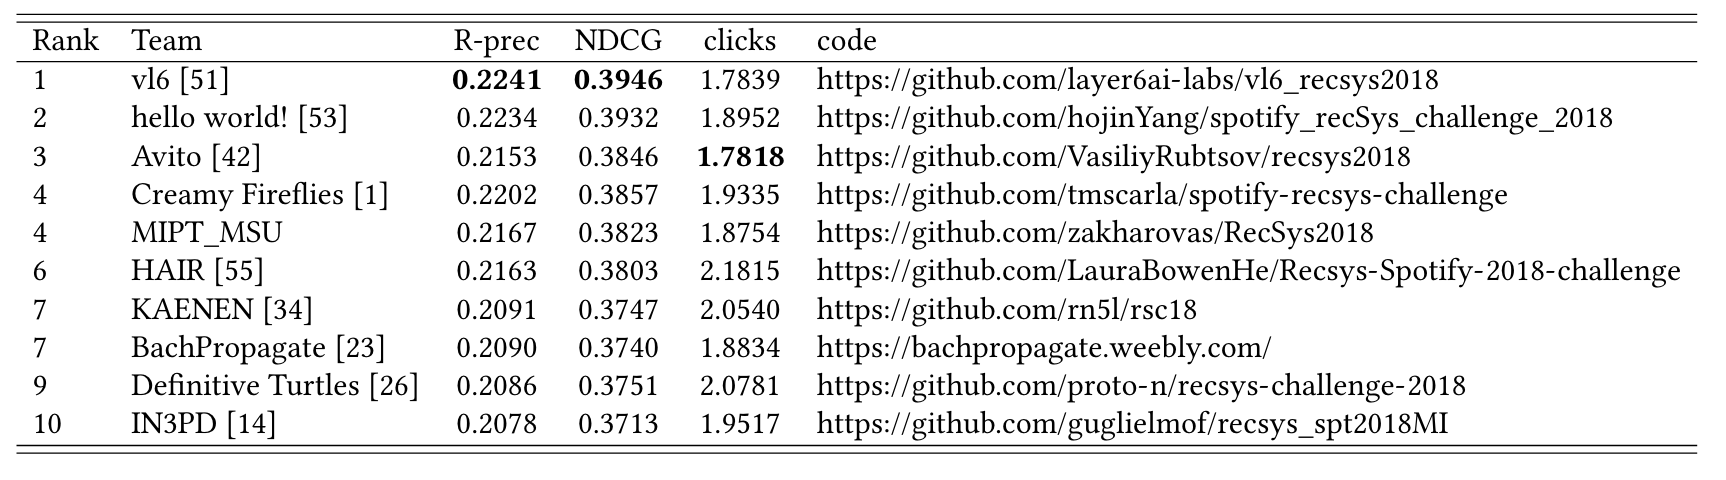
\includegraphics[scale=0.55]{images/recsys_scores}
	\caption{Top 10 Teams for RecSys 2018 and there given scores \citep{zamani_analysis_2019}} 
\end{figure}

\section{Summary}
Two experiments were conducted. First was finding the highest average r-precision value, through changing the latent factors used in the alternating least squares part of the model. After the latent factor value that obtained the highest r-precision value was found, the input song count of the DJ sets was changed. This didn't improve the average r-precision value. The highest scoring average r-precision value was compared with the top performing models of the \textit{RecSys} 2018 convention. The proposed model scored considerably lower. 
% note that \Blindocument has 5 numbered levels, despite setting secnumdepth above. I (and many style guides) would suggest using no more than 3 numbered levels (incl. the chapter), with the option of a fourth unnumbered level.

% Chapter 7
% !TEX root = ../TechProject.tex

\graphicspath{{Chapter7/}}

\chapter{Conclusions and Further Work} 

Chapter 1 identified that a dataset of  DJ sets could provide better song recommendations to DJ set centric genres compared to industry standard models. Research in this field is limited, so a simple recommendation model built around a dataset found on \textit{MixesDB} was made and an investigation on its quality was conducted. The following research questions were proposed:

\begin{enumerate}
	\item \textit{What are effective methods for the automated recommendation of songs suitable
		for adding to a given DJ set?}
	\item \textit{Is the proposed method a suitable solution for the automated recommendation of songs suitable for adding to a given DJ set?}
	\item \textit{Can a DJ-set centric dataset be used to solve other DJ tasks?}
\end{enumerate}

Chapter 2 answered Question 1 by establishing how recommendation systems worked, and the Diversity issue that baseline music recommendation systems struggle with. Chapter 3 answered Question 3 by analysing machine learning and deep learning advances and how it can be beneficial within the world of DJing. 

Chapter 4 then presents a Hypothesis that is drawn from the gaps in knowledge found in the literature review. Chapter 5 presents an overview on how the proposed application works. Chapter 6 then answers the second research question through an experiment. Chapter 7 discusses the results, and this Chapter 8 concludes the experiment and discusses how the work can be taken further.

Section 8.1 will provide a summary on how each of the chapters answered the research questions.
Section 8.2 will highlight the results found in and how it relates to the research questions proposed. Section 8.3 will describe the use of these results within the world of  recommendation systems and DJing. Section 8.4 will discuss the limitations of
this  study and  further work that could be completed is suggested.

\section{Findings of each chapter}
This section summarises how each chapter answers the research questions.

Chapter 2 analysed literature in regards to application systems and music taste to answer the following question: 

\textit{What are effective methods for the automated recommendation of songs suitable
	for adding to a given DJ set}

It was concluded that despite recent improvments in music recommendation systems, people with diverse music would often still find music in non-algoirthmic ways. And a dataset that borrowed specifically from listeners with a diverse music taste has not been explored fully.

The hypothesis goes onto highlight how this  is a problem that affects DJs specifically.
\\

Chapter 3 then examines studys in machine learning to answer the research question:
\\
\\
\textit{Can a DJ-set centric dataset be used to solve other DJ tasks?}
\\

It goes onto discuss how advancements in source separation, classification and automatic mixing can benefit the world of DJing, it also identifies a gap in research for recommendation systems aimed specifically at DJing.

An overview on how the proposed system was made. It's described how the system is built upon the work done by Daniel Chow to create a system that will work for a whole DJ sets, instead of just a single song. It's also explained how it gives more refined choice due to the use of audio features provided by the Spotify API. A few examples of inputted DJ sets are provided, with a brief description on the findings. 

\section{Main Findings of the study}

This section will go over the main discoveries of the paper and how it answers each of the research questions.

\begin{enumerate}
	\item \textit{What are effective methods for the automated recommendation of songs suitable
		for adding to a given DJ set}
\end{enumerate}

As stated previously, the most effective method would be to use the Spotify playlist continuer or the SoundCloud method, due to the performance of the proposed method not performing well on the given experiment. 

\begin{enumerate}
	\item \textit{Is the proposed method a suitable solution for the automated recommendation of songs suitable for adding to a given DJ set?}
\end{enumerate}

This question was answered with an experiment for calculating the models best R-Precision value and it was then compared with industry standard models. The optimal latent factor value was found initially and then larger DJ sets were used to see if results improved. Larger DJ sets hindered the r-precision value and the highest case scored significantly lower to competing models. However, with many areas of the experiment that could be improved, further research should still be done  around providing an automated recommendation system specifically DJ Sets.

\begin{enumerate}
	\item \textit{Can a DJ-set centric dataset be used to solve other DJ tasks?}
\end{enumerate}

Despite scoring low, the investigation provides insight on how using a concentrated dataset could better cater to specific audiences. A further developed update on this dataset and model benefit other areas of DJing . 

This only appears on a handful of mixes on \textit{MixesDB}, but a time code along with the set list could provide the foundations for a very helpful DJ tool \citep{mixesdb_2015-01-02_2015}. Hearing instances of an input song getting mixed in and out of could help speed up the learning process when they immediately have an audio reference of effective mixing. One hopes further research is done into the large extent of DJ sets available on the internet, to hopefully make DJing a more accessible pass time. 

\section{Further Work}

A recommendation system that pulls from a dataset of exclusively DJ sets was proposed to see whether it gathers more suitable solutions compared to the current industry standard models available. 

\subsection{Application}
Despite being an objectively outdated method, using collaborative filtering as the basis of the model felt appropriate due to its continued usage in modern systems. The investigations purpose was more to test the quality of recommendations being pulled from a refined dataset rather than a larger, more general dataset. All this being said, adapting the model to use deep learning with this dataset would've been a great opportunity to see whether an improved model would show more desirable recommendations.

A potential implementation was to enable user control of the recommendation process more than just choosing the input songs. It's a believable scenario where a user would appreciate the initial pool of recommendation as much as the refined selection.

The Spotify features play a big role in refining down the similar songs to those that have the most similar attributes to the input songs, allowing them to be easily incorporated into a DJ set. This proved helpful in cherry picking the best songs. 

The vectors used for euclidean distance could've been implemented better, for example, adding weights to certain attributes, such as prioritising songs at a certain BPM or key. The weighting for key could've been explored to an interesting length, by prioritising the same key but also the relative major/minor or subdominant or dominant keys.

Improvements could have been made for finding an average input vector with the Spotify features. The issue being one outlier input song could disproportion the input average and spoil the quality of the songs recommended. An example being input songs with vastly different BPM's. Ignoring outlier songs when making an input average could resolve this. Initially suggested songs most similar to the outlier input songs could then be used sparingly in the final batch.

For testing there were several ways the application could have been assessed further:
\begin{itemize}
	
\item \textbf{Recommended Song Clicks:} With \textit{Spotify} playlists, 10 songs are recommended based on what's in the playlist. The user can refresh the list and it gives out 10 more similar songs. Recommended Songs clicks is the amount of refreshes before a missing track shows up.

\item \textbf{Spotify Features:} Testing with Spotify features in conjunction with the Spotify playlist could've been done. One could input 10 songs into both the  application and a Spotify playlists. Get the Spotify features of both outputs and compare which ones are the most suitable.

\item \textbf{Spectrogram Analysis} With the dataset being linked to Spotify, a 30 second clip for each song is accessible. Assessing the input and recommended songs spectrograms would've given further insight if the songs suggested were appropriate.

\item \textbf{Listening Tests:} Gathering members of the public and getting them to listen to snippets of a given DJ set and compare the applications suggestions and industry standard suggestions would've given further insight on the subjective quality of the application.
\end{itemize}

\subsection{Dataset}
With \textit{MixesDB} growing in popularity each year, one hopes to see further exploration in using an expanded version of the dataset to cater to other DJ related tasks. With a sparsity of 99.98\% it does make sense why this model would underperform on the given experiment. An expanded dataset should be used if another investigation in this manner is conducted. 

Despite leading music streaming platforms huge libraries, there are a lot of songs, especially ones surrounding DJ sets that cannot be found on these platforms. This is apparent from the many music archive themed channels found on YouTube \citep{allen_djs_2021}.  Reasons for this is the elusive nature surrounding sub cultures that incorporates DJing in a significant way \citep{reynolds_energy_2013}. It's very common for some artist to only release content on only physical formats like Vinyl. This is motivated by a fear of opening up there culture to a majority subset, that may risk tainting a pure experience created from a select number of people \citep{wheeler_gentrification_2020}. 

Another reason for the lack of dance music on streaming is the cost of sample clearance \citep{morey_copyright_2013}. More so than other genres (aside from Rap), sampling plays a huge role in dance music. Early instances of DJ-set orientated genres like House and Techno were build on incorporating drum machines into old disco and soul records \citep{reynolds_energy_2013}. Favourable stylistic features aside, this creates a problem where the shareholders of the given samples are lawfully given the opportunity to sue a given artists a great sum of money for using there given work without permission. This means a huge amount of DJ set centric genres, pre the Digital Age has had issues being made commercially available, a highly reported instance of this is De La Souls 30 year long quest on gaining back their highly regarded musical output from the late 80's and 90's \citep{saunders_soul_2023}.

This inadvertently hinders the proposed recommendation system because it can only input and suggest songs that are also available on Spotify. Future work could include songs on YouTube as well as Spotify. YouTube contains a huge amount of songs not on standard streaming platforms. Scraping data from services like \textit{bandcamp } would also help to populate the dataset. Combining the software used to examine the Spotify features on other platforms would be beneficial, however doing this would require more processing power. The 2020 16GB MacBook Pro used for this investigation would not be sufficient.



\section{Implications}
This section will describe the implications of the data found in this investigation, with regard to the
wider context of music recommendation systems and DJing.

In the context of music recommendation systems, the data found is insignificant, but hopefully it will start a conversation around using focussed datasets to train algorithms aimed at certain audiences. This could potentially draw in audiences with an objectively diverse taste to find music in an algorithmic way.

In the context of DJing the results also are nothing to behold. However, similar to the comment made about music recommendation systems, one hopes with the mass amount of data on the internet surrounding DJ sets, it will be made use of to algorithmically automate aspects surrounding DJing. This has the potential to make DJing more approachable to newcomers. 


% note that \Blindocument has 5 numbered levels, despite setting secnumdepth above. I (and many style guides) would suggest using no more than 3 numbered levels (incl. the chapter), with the option of a fourth unnumbered level.

%% Appendices
%% appendices work in an identical way to chapters (in terms of syntax), but are labelled alphabetically rather than numerically
\appendix
% Replace "Chapter" with "Appendix"
\addtocontents{toc}{\protect\renewcommand{\protect\cftchappresnum}{\appendixname~}}
\addtocontents{toc}{\protect\addtolength{\cftchapnumwidth}{1em}}
%\input{Appendix1}
%\input{Appendix2}

% Last I checked, the Appendix and Titlesec package do not get on with each other. So use "input" for appendix chapters instead. If you still want to use \includeonly, put the \input commands in another file and \include that.

%%%%%%%%%%%%%%%%% BACK MATTER %%%%%%%%%%%%%%%%%
\backmatter

% header
\renewcommand{\chaptermark}[1]{\markboth{#1}{}}

% !TEX root = ../TechProject.tex

\graphicspath{{BackMatter/}}

\phantomsection
\addcontentsline{toc}{chapter}{References}
%% add references here
\bibliographystyle{iosrnew.bst}
%\bibliography{TechProjbib.bib} your bib file name

\bibliography{BackgroundReading.bib}
\end{document}
